\documentclass[jkps,preprint,fleqn,showpacs,showkeys]{revtex4}

\usepackage{graphicx}
\usepackage{amssymb}
\usepackage{amsmath}
\usepackage{bm}
\usepackage{lineno}
\usepackage{xspace}
\usepackage{cleveref}
\usepackage {xcolor}

\newcommand{\XGB}{XGBoost}

\begin{document}
\setcounter{page}{0}
\title[]{ MC-based feasibility study of new sampling calorimeter for measuring the $\gamma$ incident angle }

\author{YoungJun \surname{Kim}}
\author{Jung Keun \surname{Ahn}}
\affiliation{Department of Physics, Korea University, Seoul 02841}
\author{Junlee \surname{Kim}}
\email{junlee.kim@cern.ch}
\author{Eun-Joo \surname{Kim}}
\email{ejkim@jbnu.ac.kr}
\affiliation{Department of Physics education, Jeonbuk National University, Jeonju 54896}
\author{GeiYoub  \surname{Lim}}
\affiliation{IPNS/KEK Tsukuba, Japan 305-0801}

%\date[]{Received 6 August 2007}

\begin{abstract}
We present studies on the detector configuration to measure the incident angle of the $\gamma$, which has the energy ranging from hundred MeV to few GeV using a new sampling calorimeter. The sampling calorimeter consists of alternating 1-mm-thick lead sheets producing the electromagnetic (EM) shower and strips of 5-mm-thick plastic scintillators measuring the energy deposit by the shower particles. The strips are arranged along to the alternating horizontal and vertical directions to measure the transverse profile by combining the both directions at a given longitudinal position. In this paper, we used the GEANT4 to simulate energy deposit to the individual strips of the calorimeter, and the $\XGB$ to reconstruct the incident angle from energy deposits. 

The angular resolution weakly depends on the width of the strips up to 15 mm and becomes worse with the increasing width. It is found that the incident angle is reconstructed with the compatible angular resolution using front 5 radiation length of the detector. The resolution does not depend on the incident angle up to 30 degrees, and largely depends on the incident energy, which can be expressed as 0.1+1.2$/ \sqrt{E_\gamma}$.

\end{abstract}

%\pacs{68.37.Ef, 82.20.-w, 68.43.-h}
%\keywords{String shoving, Collectivity, $pp$ collision}
\maketitle

\section{Motivation}
\label{sec:mot}
The EM calorimeter has played an important role in experimental studies on the nuclear and particle physics. Various materials have been developed for better energy and timing resolution so far~\cite{Calorimeter}. On the other side, the sampling calorimeter becomes popular in the large-scale high energy experiment mainly due to its cost-effectiveness. The sampling calorimeter consists of alternating passive converters that generate the EM shower and active counters that measure the energy deposit. Since the energy deposit in the passive convert is not measured, the fluctuation of energy deposits in the converter and the counter, called sampling fluctuation, determines the energy resolution of the  calorimeter. The sampling fluctuation can be optimized by combining the converter and the counter with a specific portion. A 5-m-long cylindrical calorimeter made of alternating lead and plastic scintillating plates is an example of the sampling calorimeter~\cite{E391a_barrel}.

The layer structure of the sampling calorimeter enables us to measure the individual profile of the shower along to the beam direction, and the incident angle can be estimated by correlating energy deposits on neighboring layers. The measurement of the incident angle largely benefits the background rejection. Of particular, The incident angle will be an important tool for the KOTO experiment~\cite{KOTOproposal}.

Since the EM shower is evolving via stochastic processes, the incident angle would be reconstructed with a certain angular resolution. Energy deposits from random processes are used to reconstruct the incident angle with the machine learning, which provides better angular resolution. The evolution of the EM shower is generated with the GEANT4 and $\XGB$ was used to reconstruct the incident angle.

The sec~\ref{sec:ems} sec~\ref{sec:res} sec~\ref{sec:sum}
In the following section, the configuration of detector and Monte Carlo simulation for electromagnetic shower generation will be given. In the section III, we will describe how to reconstruct incident angle from the generated detector response by using one of the most attractive toolkit of the machine learning; $\XGB$. Finally, we will summarize our study briefly.

\section{ELECTROMAGNETIC SHOWER}
\label{sec:ems}
We started the study with a detector setup consisting of alternating lead sheet as the passive converter and strips of the plastic scintillator as the active counter. The thickness of lead is 1 mm and scintillator is 5 mm, respectively. The lead sheet has a cross-section of  500 mm $\times$ 500 mm and each scintillator strips of 500 mm $\times$ 15 mm  being arranged along the X- and Y-direction alternatively along Z-direction as shown in  Fig.~\ref{fig:det_conf}. Total number of alternating layers is 105 which corresponds to 20 radiation length (20 Xo) and possible to contain all of the shower particles generated by $\gamma$ in the region of medium energy (from  100 MeV to few GeV). 
 
\begin{figure}[!hbt]
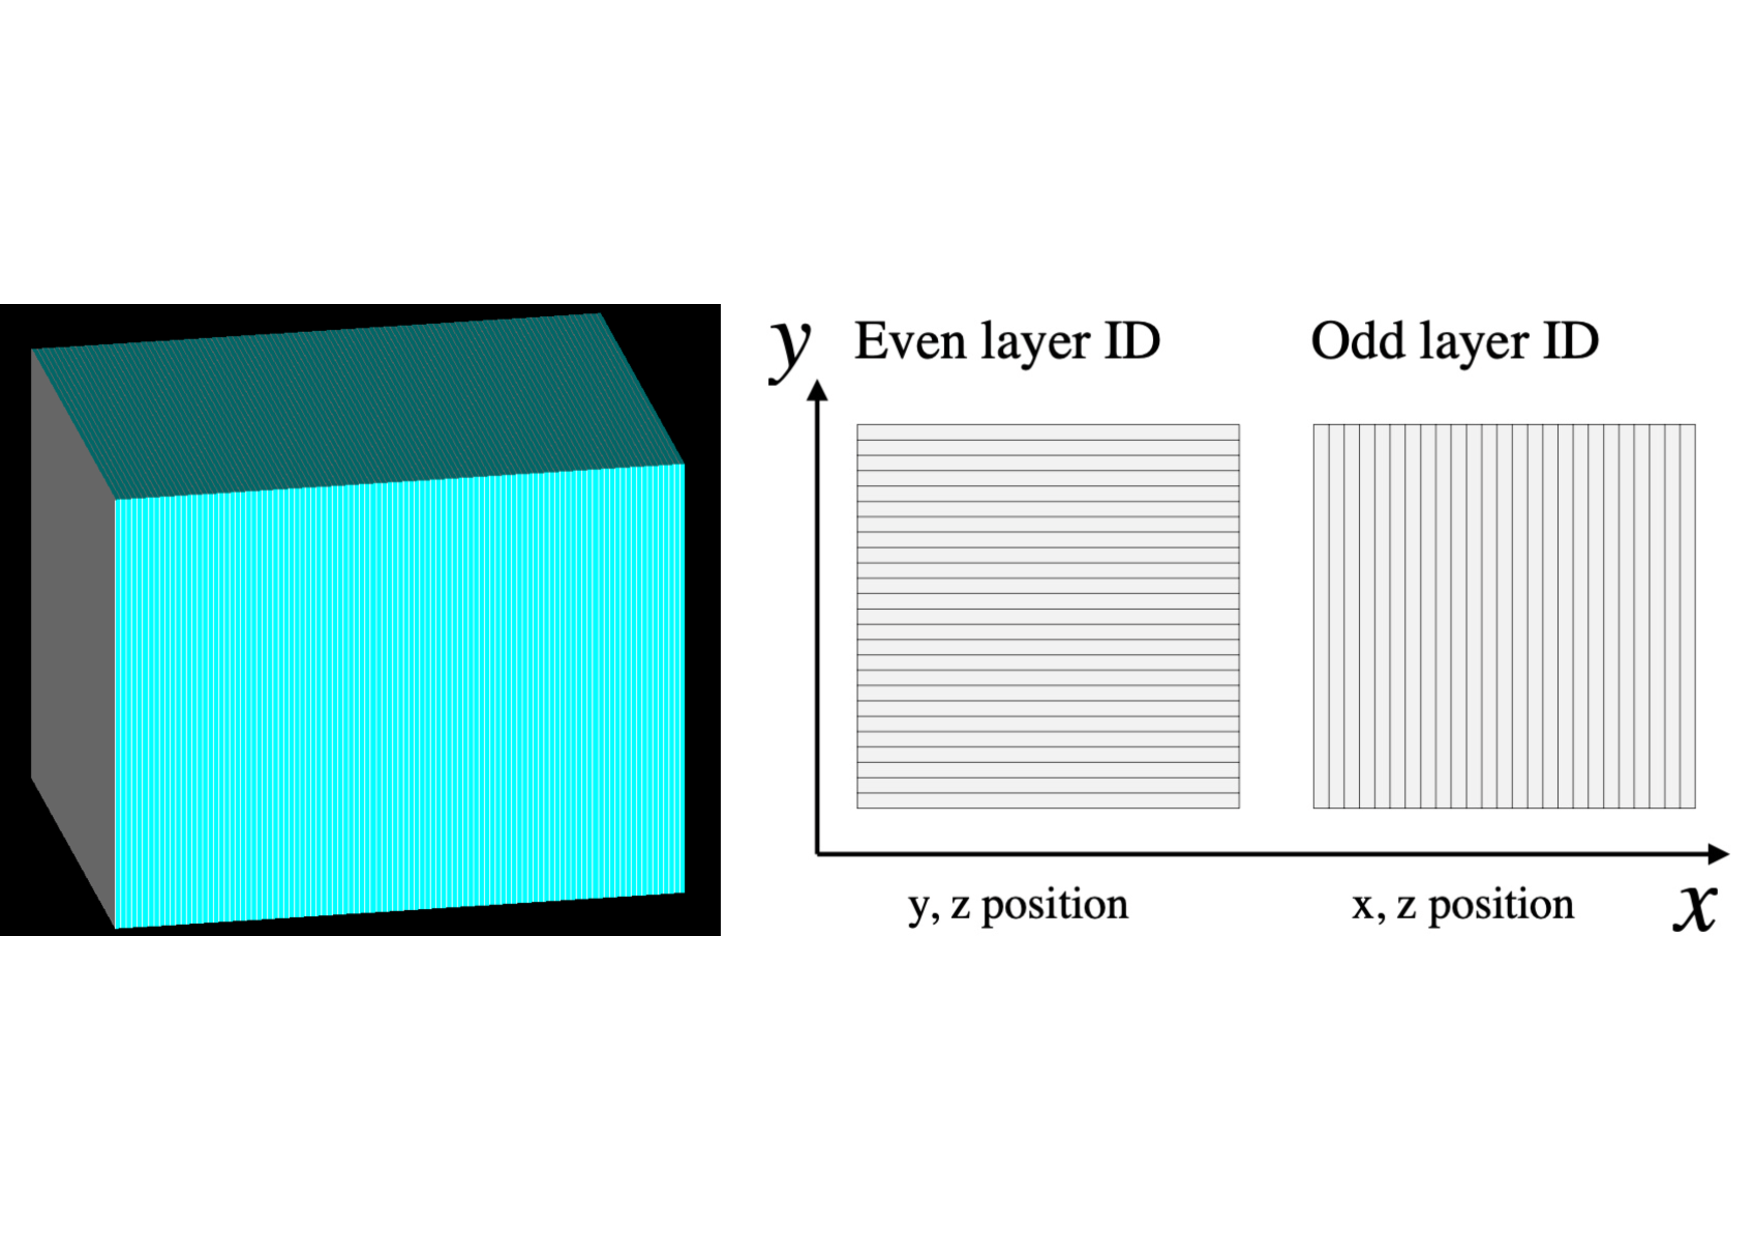
\includegraphics[width=0.85\textwidth]{figures/Sec2/Prototype_samplingcal.pdf}

\caption{ The first trial of detector setup for simulation study on angle measurement. It is a sampling calorimeter consisting of alternating lead sheets and strips of plastic scintillator. }
\label{fig:det_conf}
\end{figure}

The generation of incident $\gamma$ and its interaction with detector materials was simulated by using the GEANT4 package (ver. xxx) with the standard EM sub-packages~\cite{GEANT4}.
The $\gamma$ entered the center of the detector and moved to the positive direction of Z-axis, where the surface of the first layer is defined as a starting point (Z=0). Its incident angle is defined as the polar angle ($\theta$) along to the Z-direction, that is, $\theta = 0$ for the $\gamma$ enters perpendicular to the detector surface. %The generated energies are in range from hundred MeV to few GeV which is interested to the KOTO experiment. 
Figure~\ref{fig:Evt_Dis} shows a typical event display describing the energy deposit to the each scintillator strips in both of X-Z and Y-Z plane for 1-GeV $\gamma$ entering in perpendicular to the center of the detector ($\theta=0$ and $\phi=0$).


\begin{figure}[!hbt]
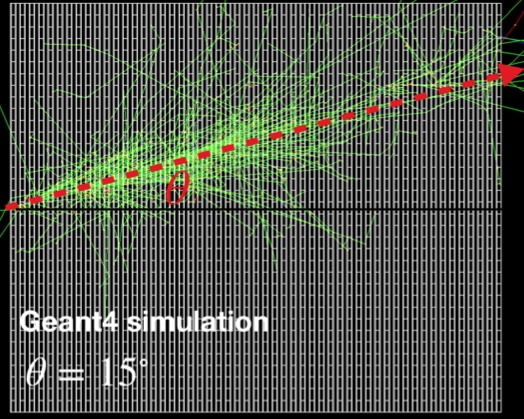
\includegraphics[width=0.45\textwidth]{figures/EventDisplay.jpg}
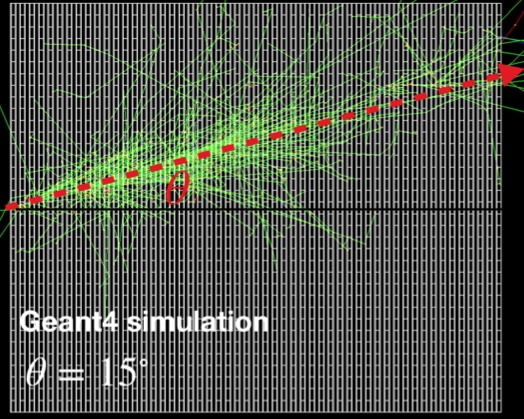
\includegraphics[width=0.45\textwidth]{figures/EventDisplay.jpg}
\caption{Distribution of energy deposit to the each scintillator strips in X-Z plane (Left) and Y-Z plane (Right) for 1-GeV $\gamma$ entering perpendicularly to the detector ($\theta=0$ and $\phi=0$).}
\label{fig:Evt_Dis}
\end{figure}

The GRANT4 can provide reliable results on the electromagnetic shower produced by the incident $\gamma$. Its longitudinal profile depends on incident energy and can be expressed \cite{Longo} by the three parameters as following;
\begin{equation}
    F(E,t)=A  t^\alpha e^{-bt},
\end{equation}
where t is the position of scintillator strips along the Z-direction. As shown in Fig.~\ref{fig:Longitudinal}, the Eq. 1 describes the obtained average energy deposit on each layer of scintillator strips reasonably. In the case of the sampling calorimeter, however, the energy deposit on the converters and counters is caused by multiple processes and its fraction is changed along with the shower develpoment.

As a result, the ratio of the energy deposit in counter and in converter changes according to the layer position as shown in Fig.~\ref{fig:Longitudinal} (right). In order to describe the shower profile in the sampling calorimeter, we need to take into account the layer dependent of the energy deposit. Since we will use the simulated results only for current study on angle measurement, we did not proceed any further analytic study on the process.

\begin{figure}[!hbt]
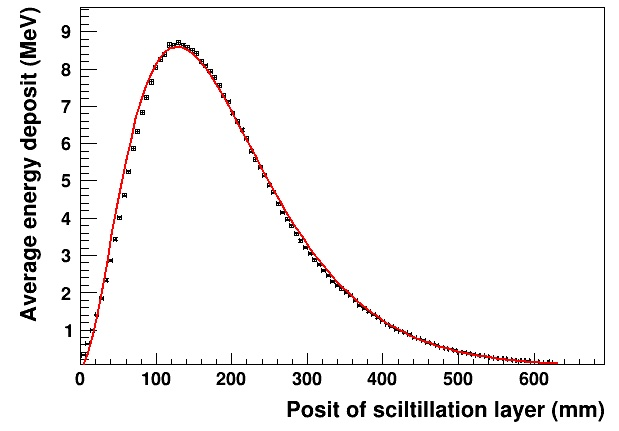
\includegraphics[width=0.48\textwidth]{figures/LongProfile.jpg}
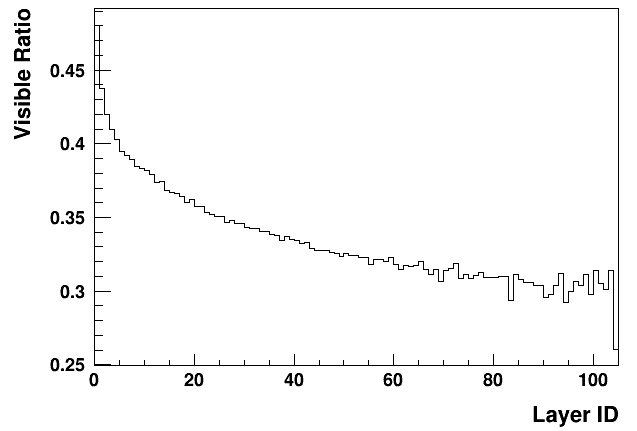
\includegraphics[width=0.48\textwidth]{figures/LayerVisibleRatio.jpg}+
\caption{Generated average energy deposit on the scintillator strips along Z axis(left) and visible ratio for each layer.}
\label{fig:Longitudinal}
\end{figure}

On the other hand, the lateral spread of the shower
%is interpreted as a distribution of energy deposit in crossing positions of the X- and the Y-strips in neighbouring two layers.  This spread 
is expressed as the the Molière radius defined ~\cite{PDG} as 
\begin{equation}
R_M= 21.2~{\rm MeV}\cdot X_0 /E_c,
\end{equation}
where $X_0$ is the radiation length and $E_c$ is the critical energy of the detector, respectively. 
Since the sampling calorimeter contains different materials placed at the different localized positions, we defined the $R_M$ as the radius of cylinder containing 90\% of the energy deposit instead of using the Eq. (2). The left panel of Figure~\ref{fig:Moliere_vis} shows energy deposit per each layer (black line) and integrated energy deposit up to the layers. We can deduce the Molière radius as 70 mm, which is largely depends on the position of its measurement. The right panel of Figure~\ref{fig:Moliere_vis} shows the radius as a function of scintillator layer, which increases along the shower depth. The first three bins show large radius because of large contribution of shower particles generated opposite to the incident direction.    

\begin{figure}[!hbt]
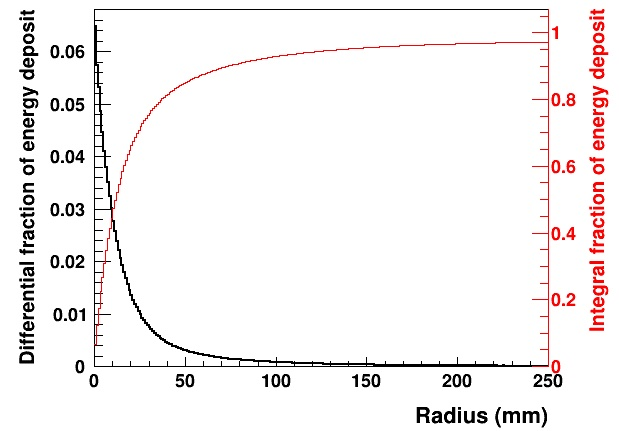
\includegraphics[width=0.44\textwidth]{figures/Edep_R.jpg}
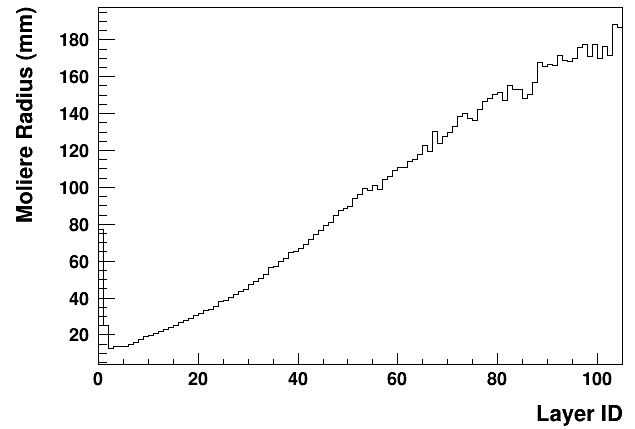
\includegraphics[width=0.48\textwidth]{figures/Moliere_layer.jpg}
\caption{Left:Energy deposit for given radius as a differential(black line) and integral distribution(red line) Right: Moliere radius as a function of ID of scintillator-strip layers.}
\label{fig:Moliere_vis}
\end{figure}

With the detector configuration shown in Fig.~\ref{fig:det_conf}, we can get three dimensional information on the showers. By using the obtained data as an input of the machine learning package, we can extract the incident angle of the $\gamma$ as explained following section. 
%When we apply the three dimensional information on the generated shower profile, we can reconstruct incident $\gamma$ more correctly by integrating the energy deposit. 
%For simplicity in numerical calculation, %For the sampling calorimeter consisting of different materials, 
%let us define the Molière radius as the radius of cylinder containing 90\% of shower energy. As shown in Fig.~\ref{fig:Moliere_vis}, the configuration of 1-mm lead and 5-mm scintillator shows $\rho_M=70$ mm in average which changes with the shower depth. %That is, we can expect an improvement on separating two gammas closely incident to the calorimeter. We will study on this subject and not discuss any more in this paper.
%the For the detector consisting of 1mm lead and 5mm plastic scintillator contain 90\% of energy deposit inside the cylinder of radius of $\rho_M=70$ mm. %It had better to compare with CsI crystal

%The energy resolution of the sampling calorimeter is mainly determined by the fluctuation of the visible ratio defined as 
%\begin{equation}
%R = { \frac{E_{act}} {E_{act}+E_{pas}}},
%\end{equation}
%where $E_{act}$ and $E_{pas}$ are energy deposit to the active and passive part of the calorimeter, respectively. This visible ratio is roughly given by the ratio of material budget between the converter and the counter. 
%is simply given by the fraction of the active component to that of the passive component, and its fluctuation becomes large when the ratio is small.
%by thickness of the converter. It is because the energy deposit at the active component is done through not only passage of the electron-positron pair but also low energy process such as compton scattering not reach to the active counter. 
%As shown in Fig.~\ref{fig:energy_res}, the mean of the visible ratio for the configuration of 1-mm lead and 5-mm scintillator is  0.35 and its energy resolution is expected 4\% for 1 GeV photon. However, the visible ratio can be improved with the same amount of composed materials when we use thinner layers. Figure YYY shows the change of the visible ratio for the same ratio $R=t_{lead}/t_{scin}$=0.2 according to the thickness of the converter (thinner scintillator too). When we make the lead sheet thinner as a factor of 5, the visible ratio improves as XXX. This is because the number of low energy electrons and positrons penetrating the lead sheet is increased in case of thinner converter. As a result of the increasing probability, the sampling fluctuation becomes small and the energy resolution improved as a result.
%This energy resolution is improved as a result thinner converter and counter keeping the visible ratio constant.

%\begin{figure}[!hbt]
%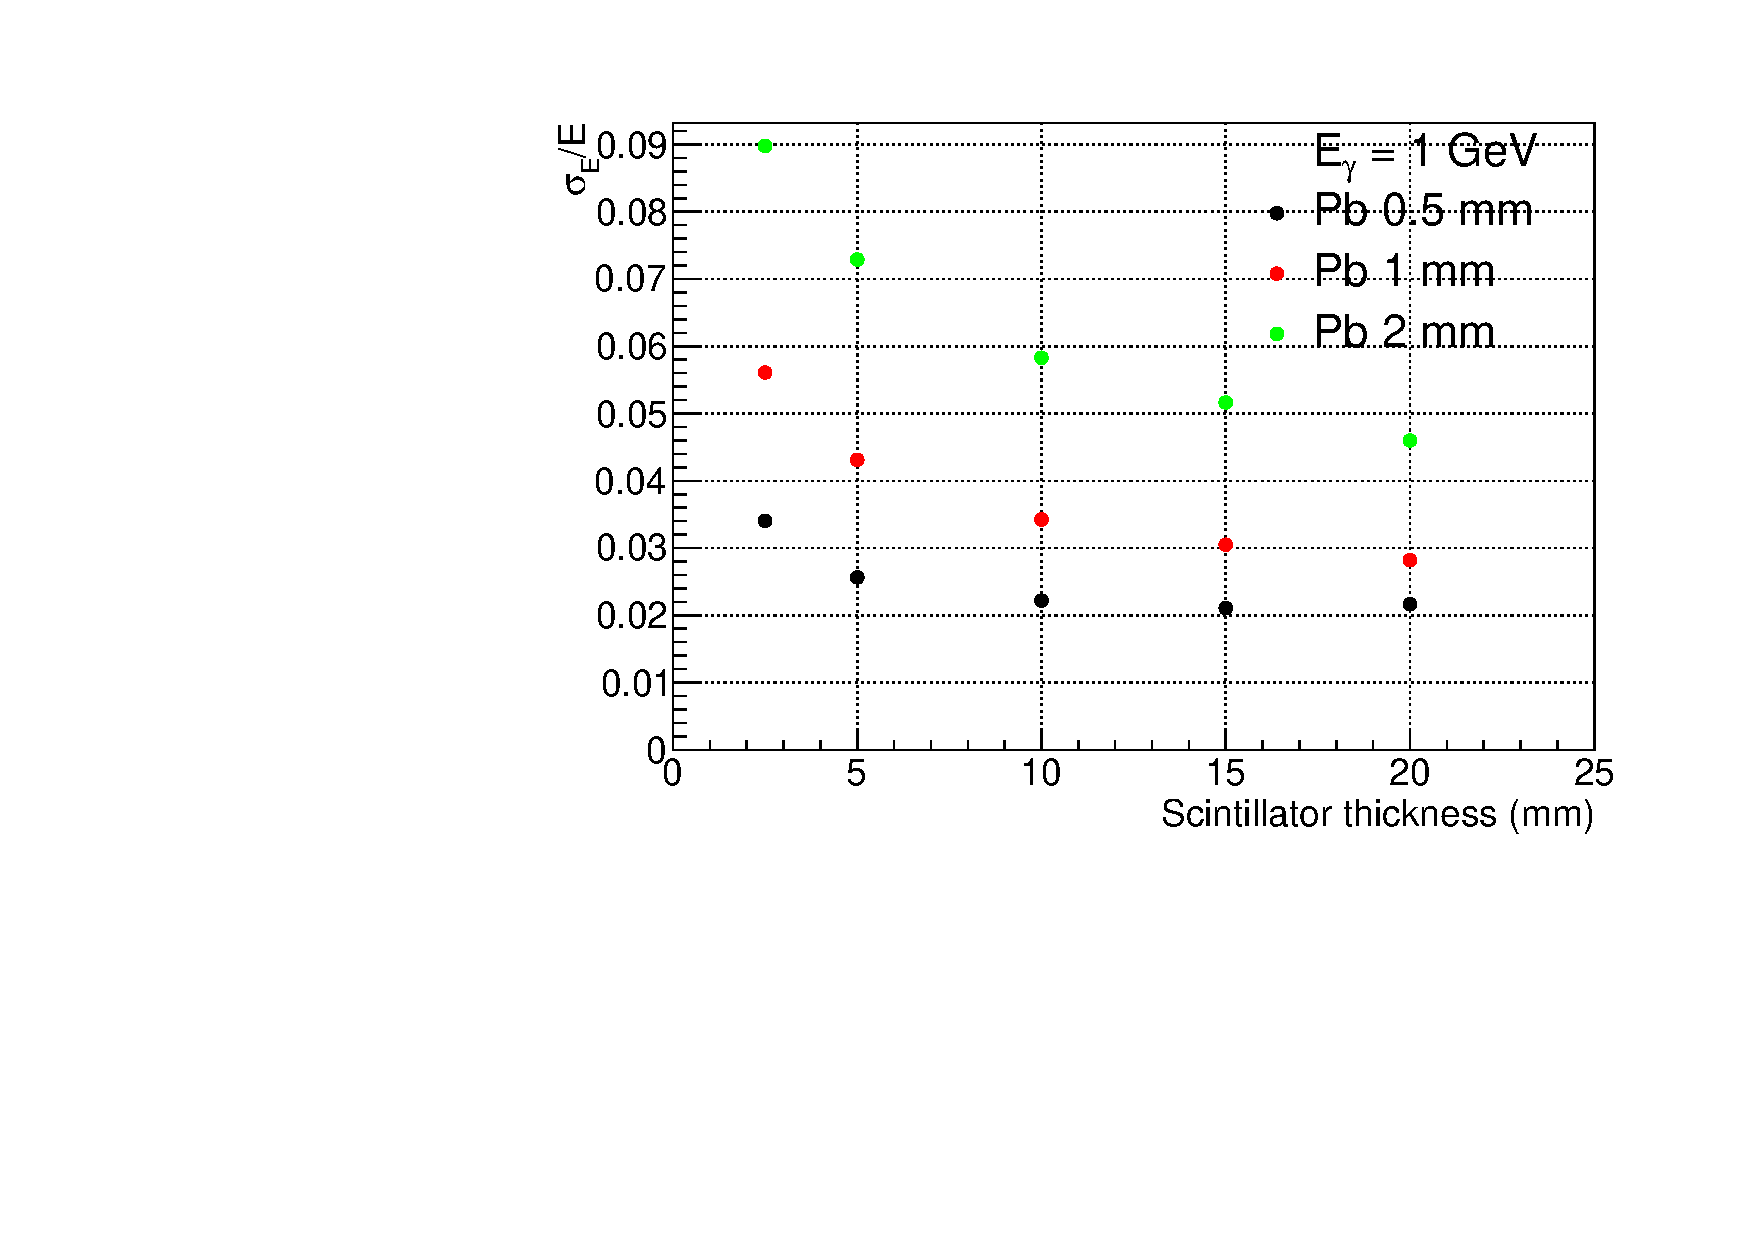
\includegraphics[width=0.48\textwidth]{figures/3.2/eres_thickness.pdf}
%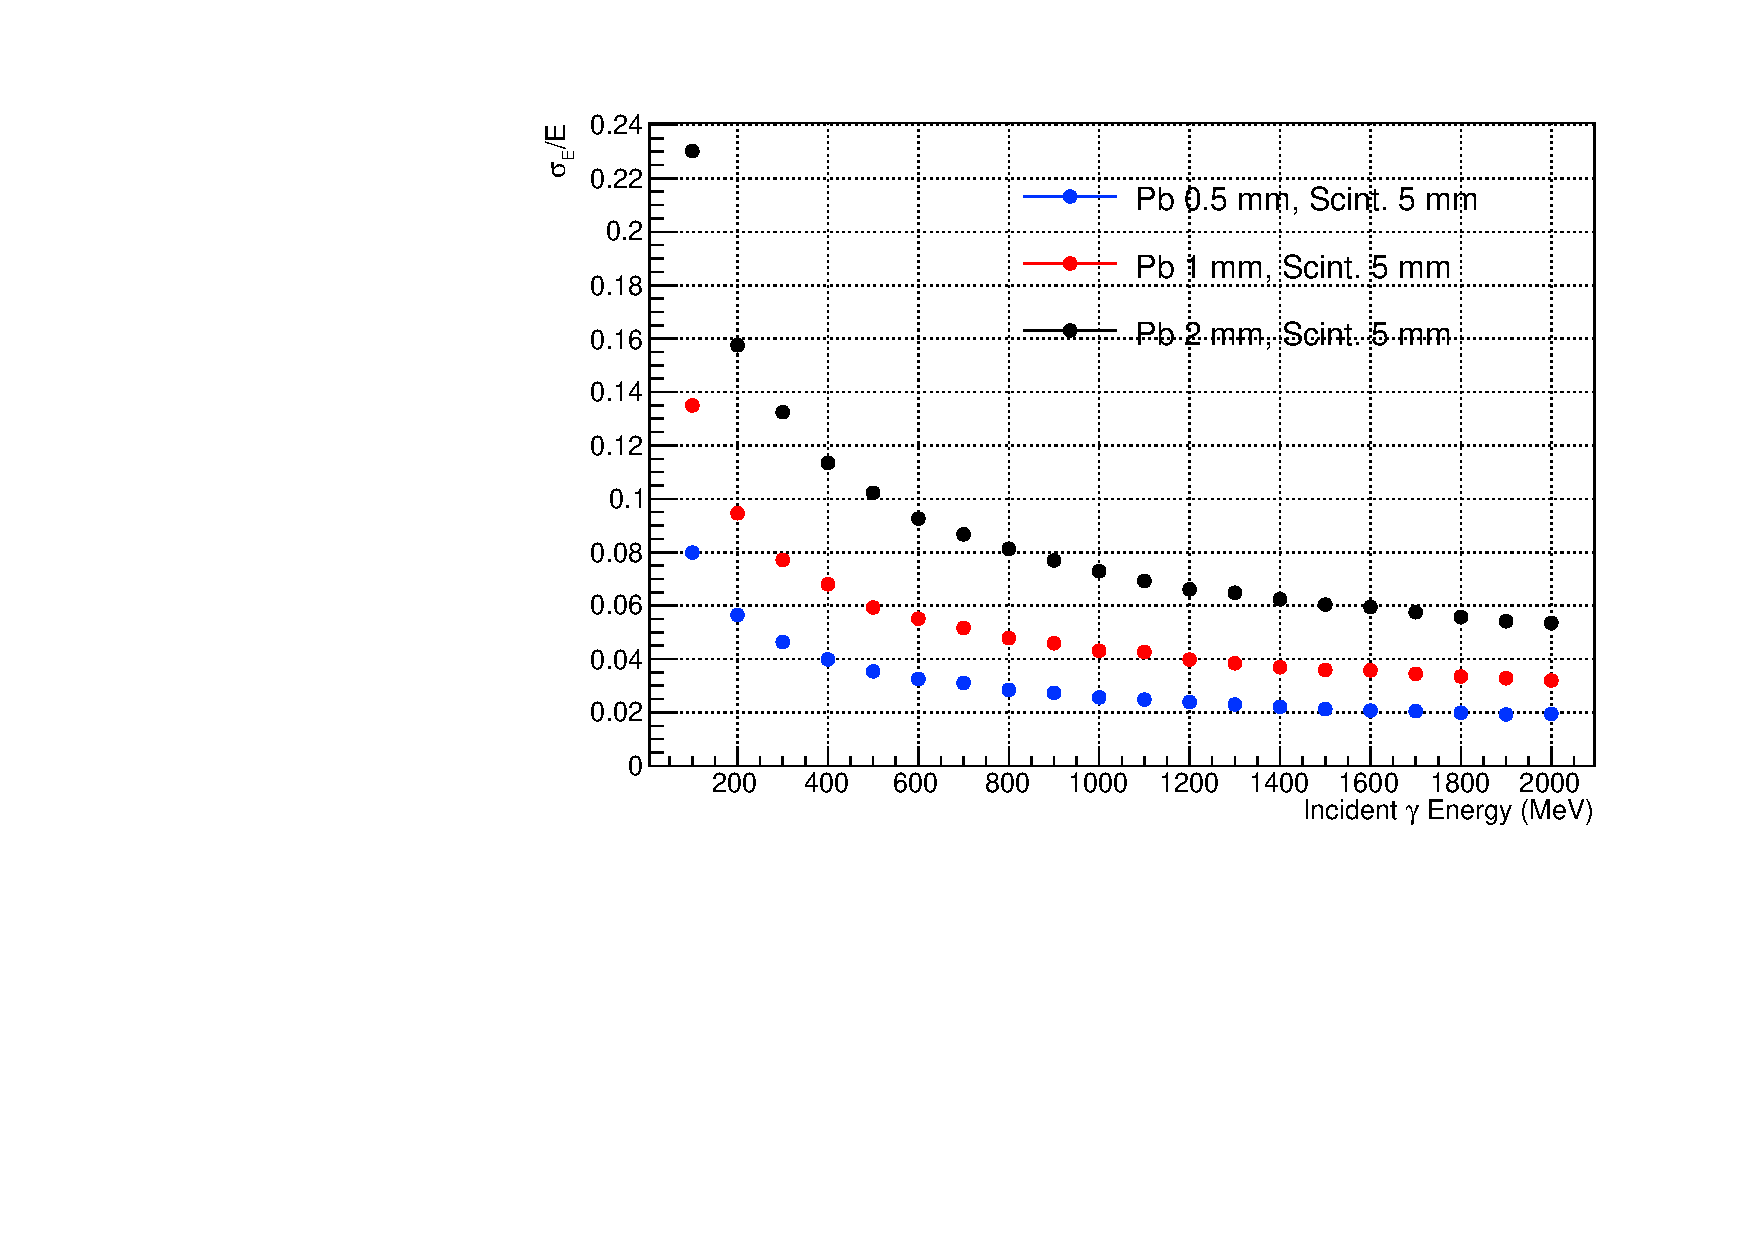
\includegraphics[width=0.48\textwidth]{figures/3.2/energy_resolution.pdf}
%\caption{Visible ratio of the sampling calorimeter for different configuration (Left) and energy resolution as a function of incident $\gamma$ energy (right).}
%\label{fig:energy_res}
%\end{figure}





%\section{Method}
We started the study with a setup of sampling calorimeter consisting of alternating lead sheet and strips of the plastic scintillator as shown in Fig.~\ref{fig:det_conf}. The electromagnetic shower mainly generated at the lead sheet (passive component) due to its short radiation length ($X_0 = 5.6~{\rm mm})$ and the information of the shower particles is obtained by using the scintillator (active  component). The thickness of lead is 1 mm and scintillator is 5 mm, respectively. The lead sheet has a cross-section of  500 mm $\times$ 500 mm and the scintillator strip of 500 mm $\times$ 15 mm. By arranging the strips in X- and Y-direction alternatively along Z-direction. The generated photon moves along with Z-direction and its incident angle was defined as a polar angle to the direction.  With the configuration, we can get shower profiles in X- and Y-axis in turn, and estimate the incident angle from them. The number of alternating layers is 105, corresponding to 20 radiation length (Xo), in order to contain shower particles fully. 

\begin{figure}[!hbt]
%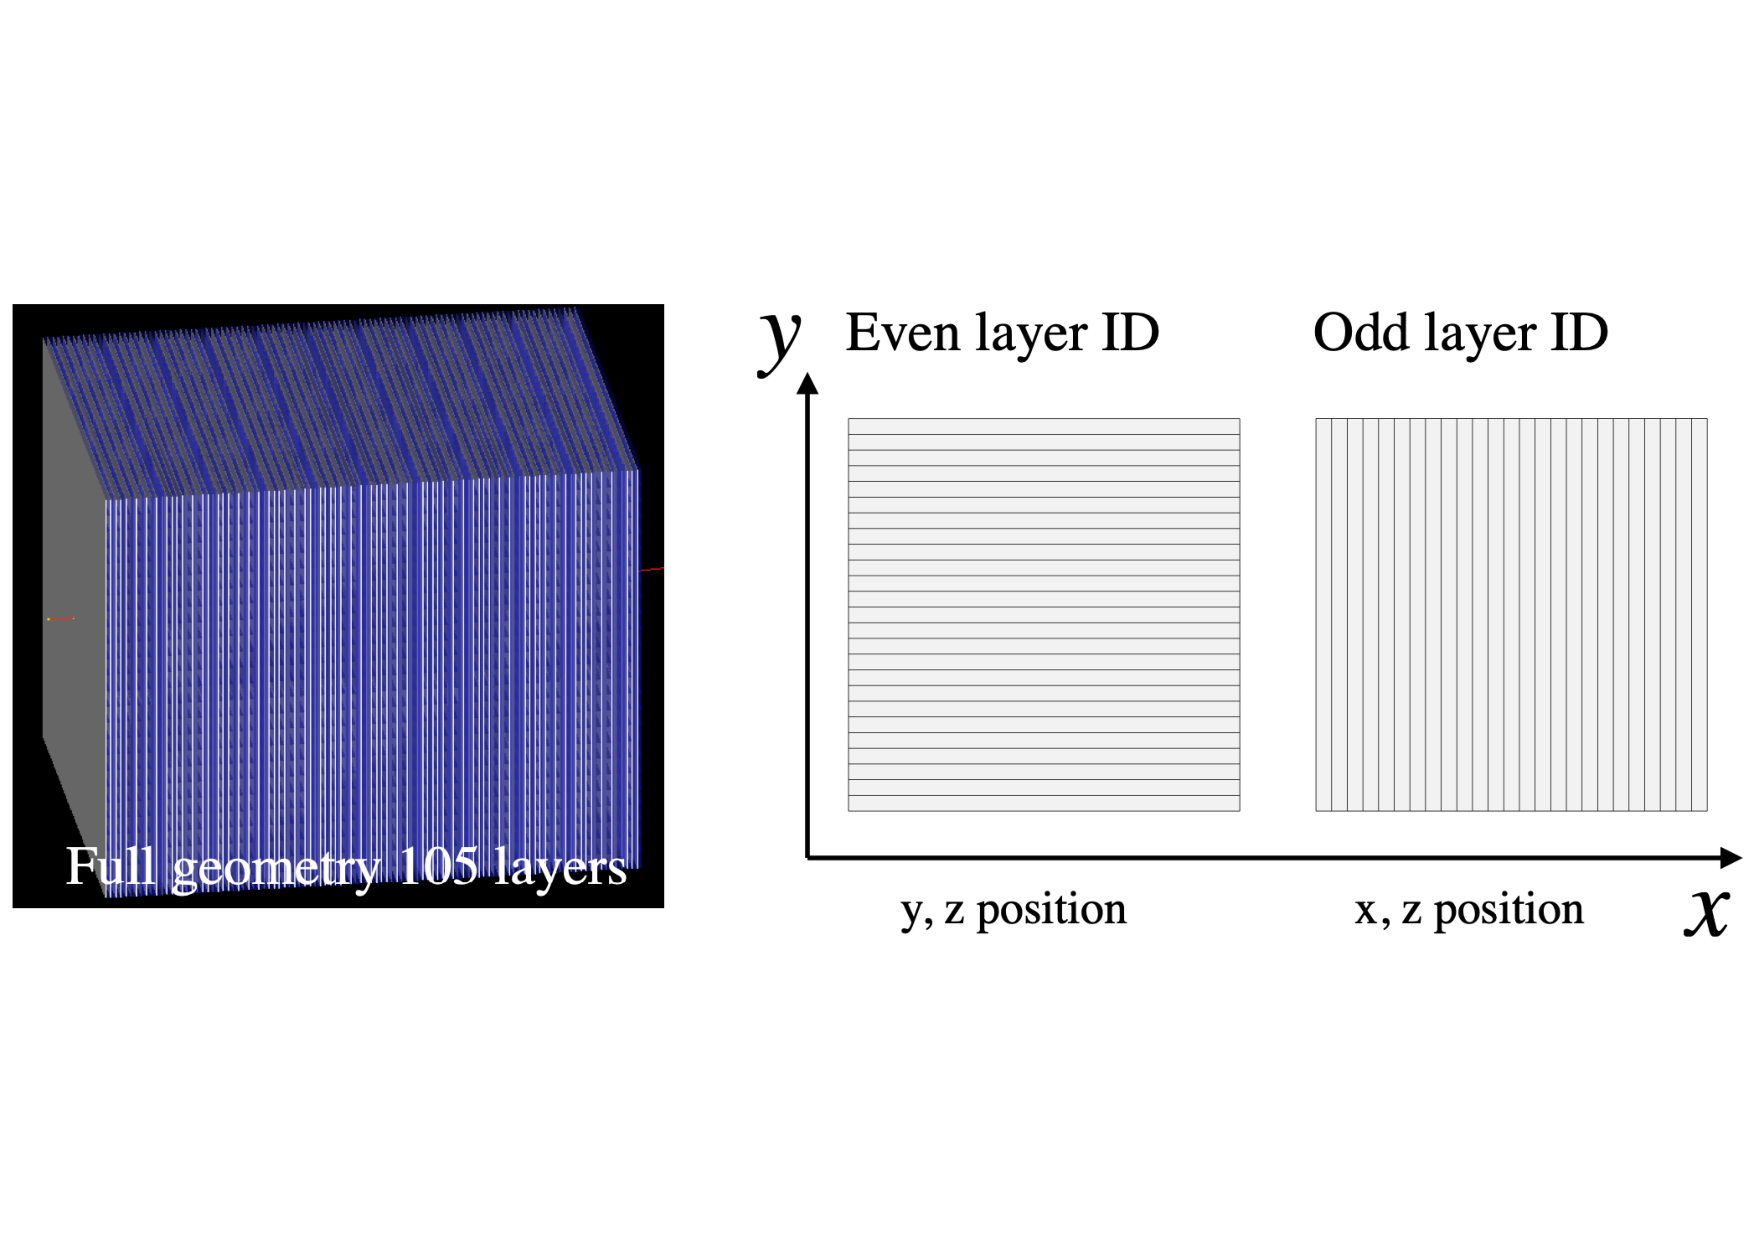
\includegraphics[width=0.85\textwidth]{figures/Sec2/ang_conf.pdf}
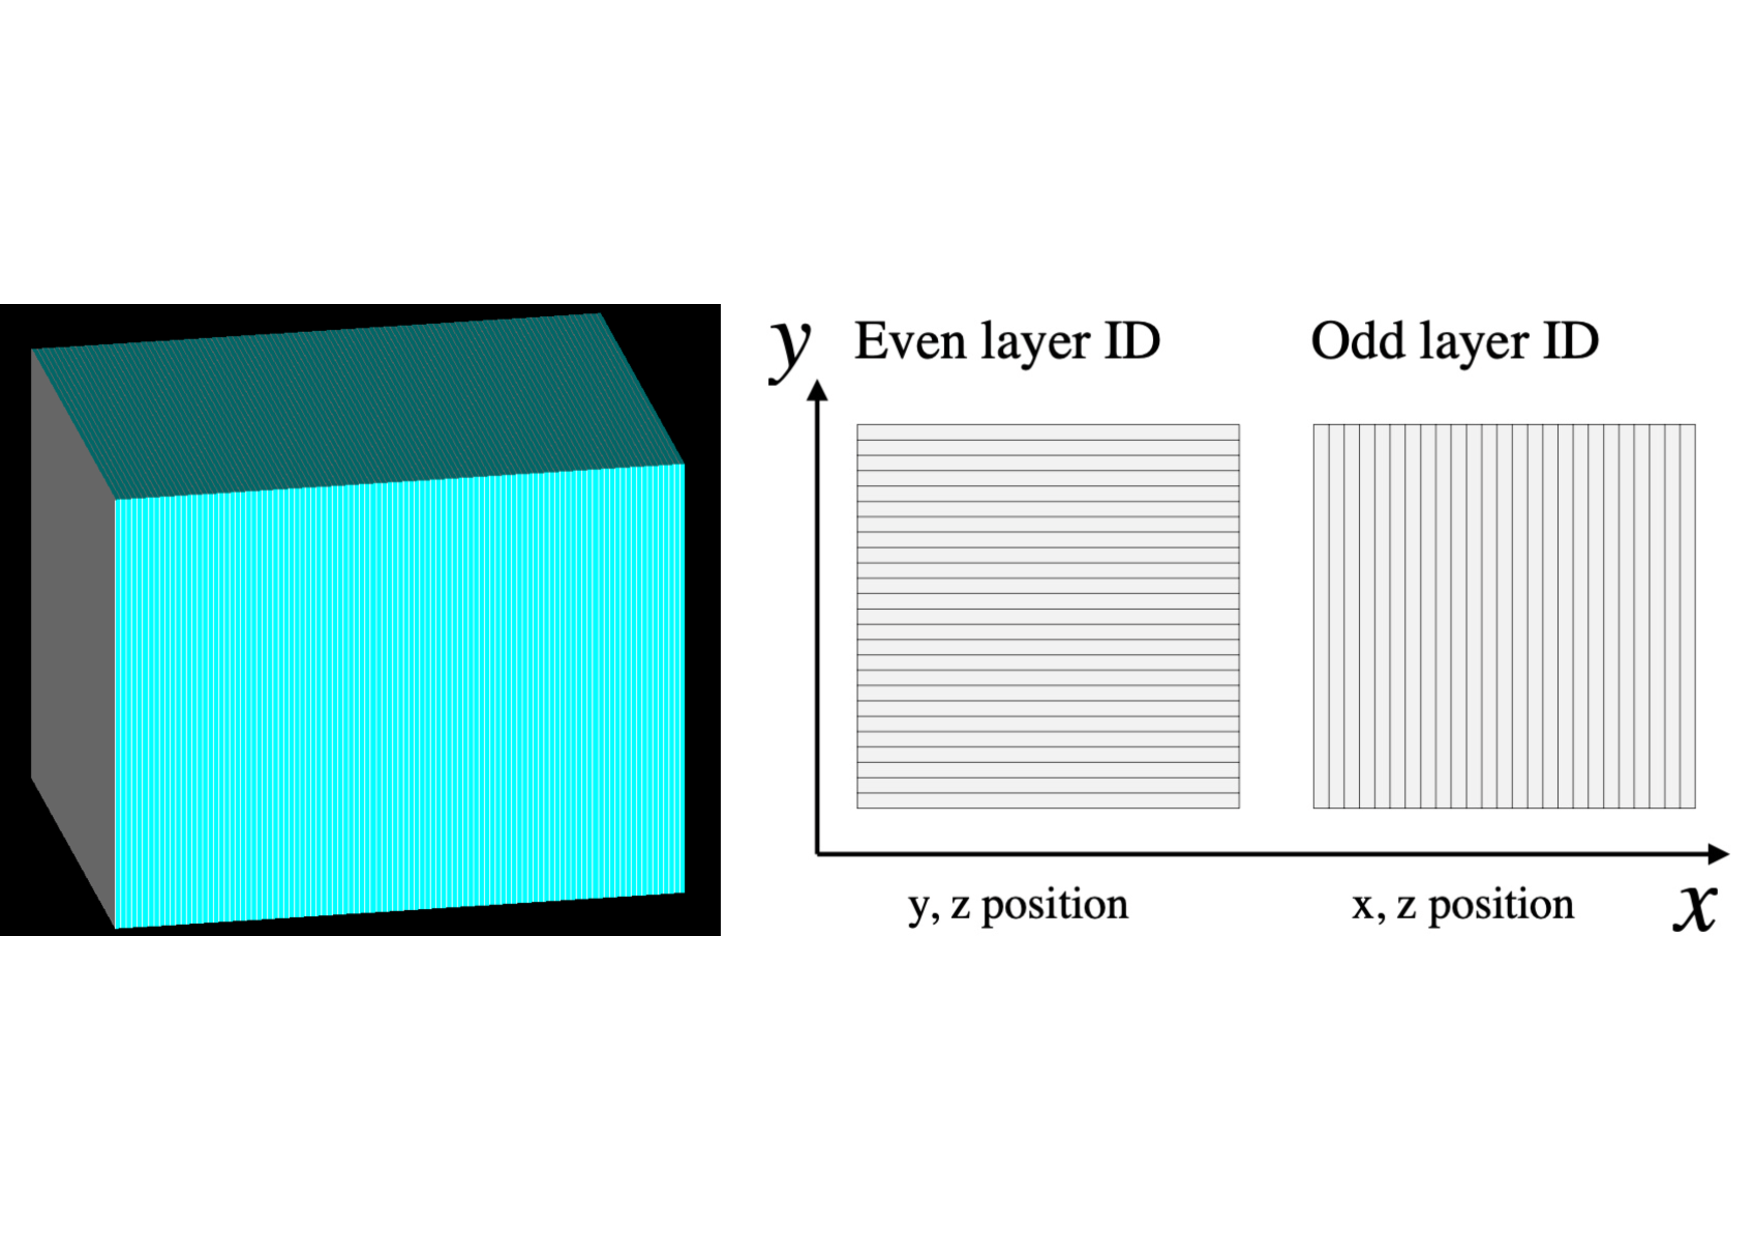
\includegraphics[width=0.85\textwidth]{figures/Sec2/Prototype_samplingcal.pdf}

\caption{ The first trial of detector setup for simulation study on angle measurement. It is a sampling calorimeter consisting of alternating lead sheets and strips of plastic scintillator. }
\label{fig:det_conf}
\end{figure}

The electromagnetic showers are generated with given detector setup by using the GEANT4 package (ver. xxx) with the standard EM sub-packages (URL: https://geant4.web.cern.ch/node/1828). 
${\it I will describe the coordinator}$
%The contribution of the hadronic interaction is taken into account with $\rm{FTFP\_BERT}$ package. The materials used in detector construction are selected from the Geant4 NIST material database: $\rm{G4\_Pb}$ for the lead and $\rm{G4\_PLASTIC\_SC\_VINYLTOLUENE}$ for the scintillator material.

In order to reconstruct the incident angle of the gamma, we used the $\XGB$, which is one of the machine learning packages supporting a scalable tree boosting system~\cite{xgboost:2016}. Input data for the $\XGB$ are deposit energies on each scintillator strip by the generated shower particles. It includes the strips of zero-energy deposit in order to satisfy the requirement that the number of input data should be identical. As the training procedure, the $\XGB$ studies profiles of energy deposit to the individual strips with respect to the incident angle for a given $\gamma$ energy. 

There are five hyperparameters which can be set by user, and their values are selected to provide the better angular resolution as described in tab.~\ref{tab:XgbPar}. Among these hyperparameters, the Max. depth rapidly improves the angular resolution with increasing its value until 100. The N\_estimators also improves the angular resolution with increasing its number up to 1,000 and N\_estimators larger than 1000 does not change the resolution. Its optimal condition becomes 1000 with the Max. depth is 100.

\begin{table}[hbt!]
\centering
\caption{Parameterization of the $\XGB$}
\begin{tabular}{cccc}
\hline 
Parameter & Function & Default value & Used value \\ \hline 
N\_estimators & The number of decision trees & N.A. & 1000 \\  
Max. depth & Possible maximum depth of tree structure & 6 & 100 \\ 
Subsample & Fraction of total data used for a single decision & 1 & 1 \\ 
Learning rate & Step length for calculation & 0.3 & 0.08 \\ 
Gamma & Requirement on minimum loss function & 0 & 0 \\ 
\hline
\end{tabular}
\label{tab:XgbPar}
\end{table}

For the training procedure, gammas are generated uniformly in the range 0 to 50 degrees of polar angle ($\theta$) and  0 to 360 degrees of azimuthal angle ($\varphi$). The performance of the angular reconstruction is tested with independently generated data samples with fixed $\theta$ and uniform $\varphi$ from 0 to 360 degrees.


%\section{method}
%\label{sec:ana}

%\subsection{Geant4 simulation}
%In this paper, the photon shower and corresponding detector responses, the prerequisites for the machine learning inputs, are simulated based on the Geant4 framework. Among several physics packages, the $\rm{FTFP\_BERT}$ physics package is used for electromagnetic and hadronic interactions as it is generally recommended for the high energy physics calorimetry. 

%The materials used in detector construction are selected from the Geant4 NIST material database: $\rm{G4\_Pb}$ for the lead and $\rm{G4\_PLASTIC\_SC\_VINYLTOLUENE}$ for the scintillator material.

%\subsection{Detector construction}
%We constructed a prototype sampling electromagnetic calorimeter with alternative stacking of thin Pb sheets and scintillator strips. A Pb sheet has a dimension of 50 cm (w) $\times$ 50 cm (l) $\times$ 1 mm (t). And a single layer of scintillator plate consists of 25 long scintillator segments, and each segment has a dimension of 2 cm (w) $\times$ 50 cm (l) $\times$ 5 mm (t). The full geometry consists of 105 layers  which is corresponding to 20 $X_0$. In order to investigate the detector properties and test the reconstruction performance of the indicent angle of $\gamma$, we generated $\gamma$ beam data samples with several incident angles and energies.
%In this study, we utilized a physics package $FPFT\_BERT$ for the hadronic and electromagnetic interactions
%We started the study with a setup of sampling calorimeter consisting of alternating lead sheet and strips of plastic scintillator as shown in Fig.~\ref{fig:det_conf}. The thickness of lead is 1 mm and scintillator is 5 mm, respectively. The lead sheet has a cross-section of  500 mm $\times$ 500 mm and the scintillator strip of 500 mm $\times$ 15 mm. By arranging the strips in X- and Y-direction alternatively along Z-direction. The generated photon moves along with Z-direction and its incident angle was defined as a polar angle to the direction.  With the configuration, we can get shower profiles in X-Z and Y-Z planes in turn, and estimate the incident angle from them. The number of alternating layers is 105, corresponding to 20 radiation length (Xo), in order to contain shower particles fully. 

%\begin{figure}[!hbt]
%%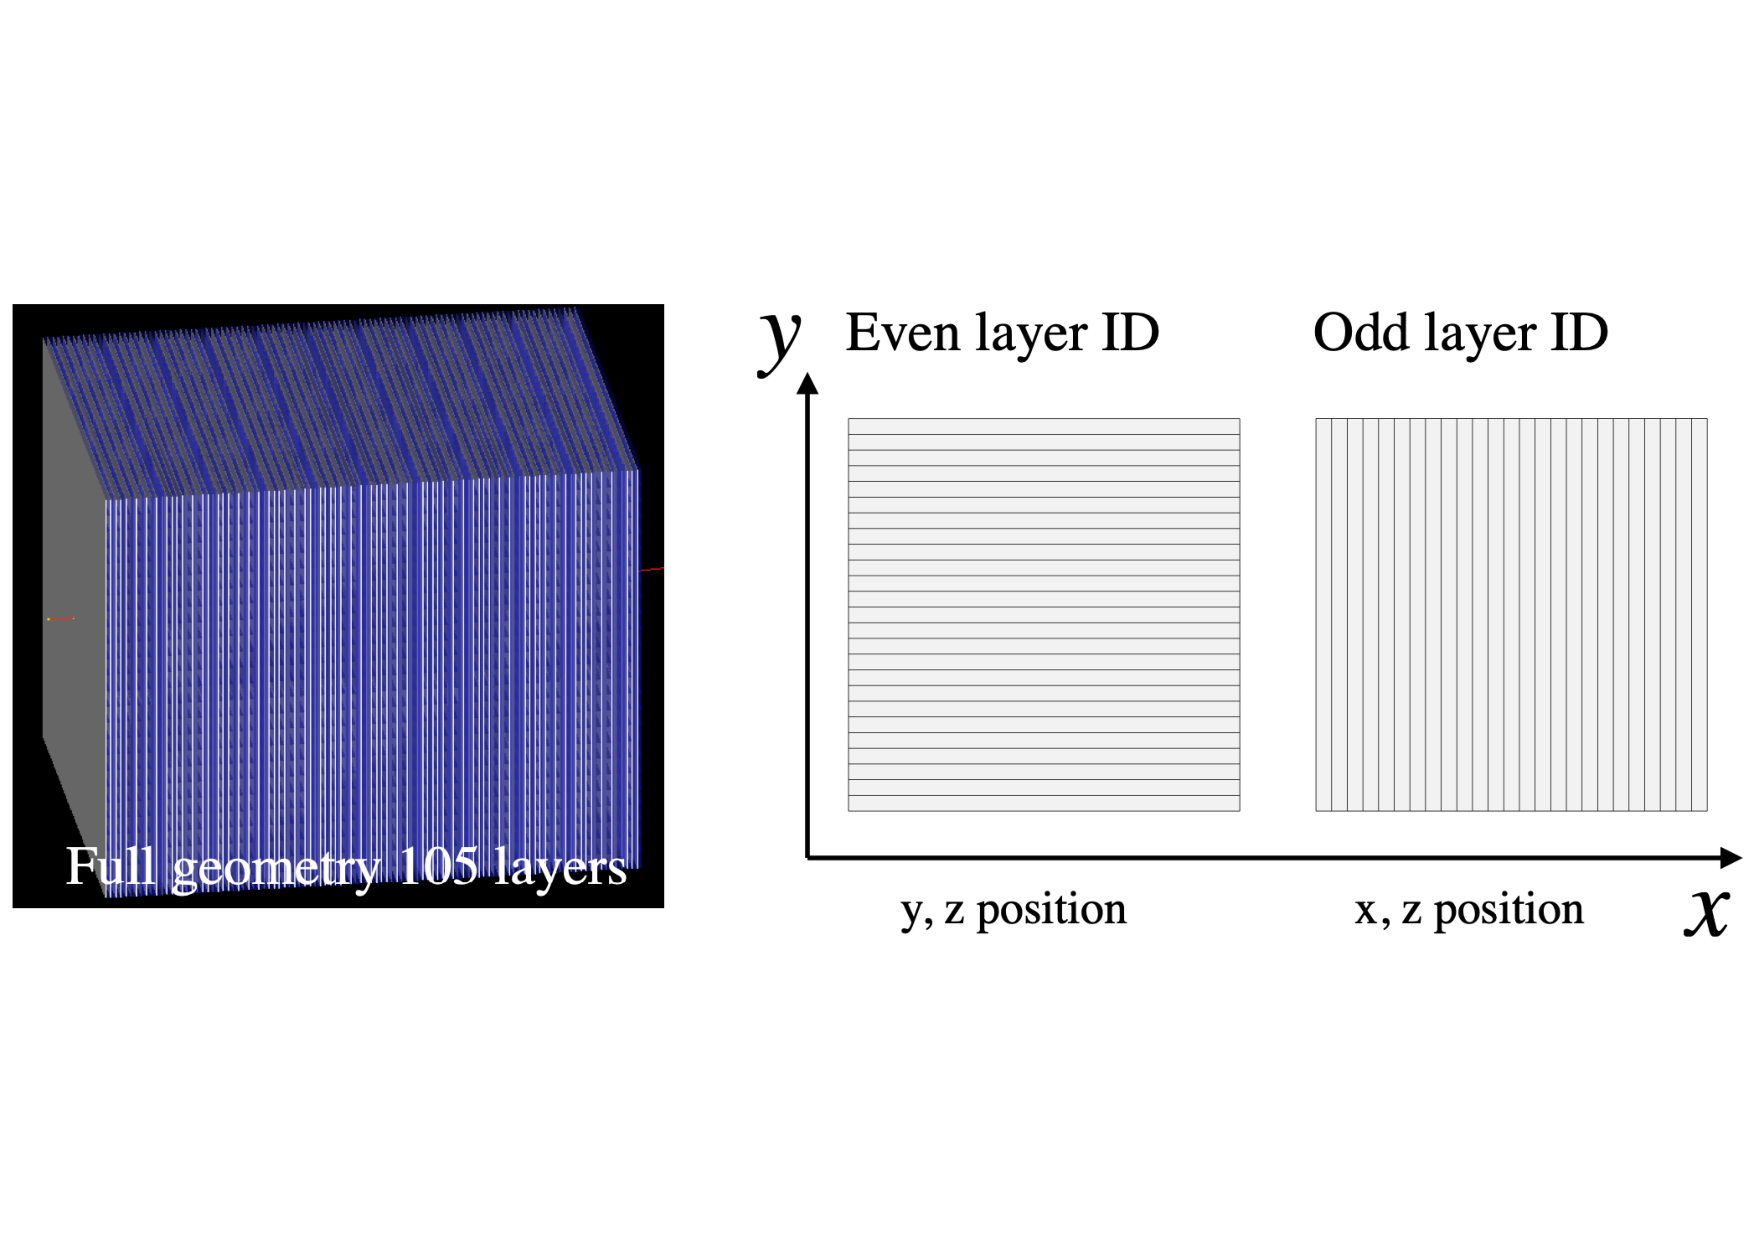
\includegraphics[width=0.85\textwidth]{figures/Sec2/ang_conf.pdf}
%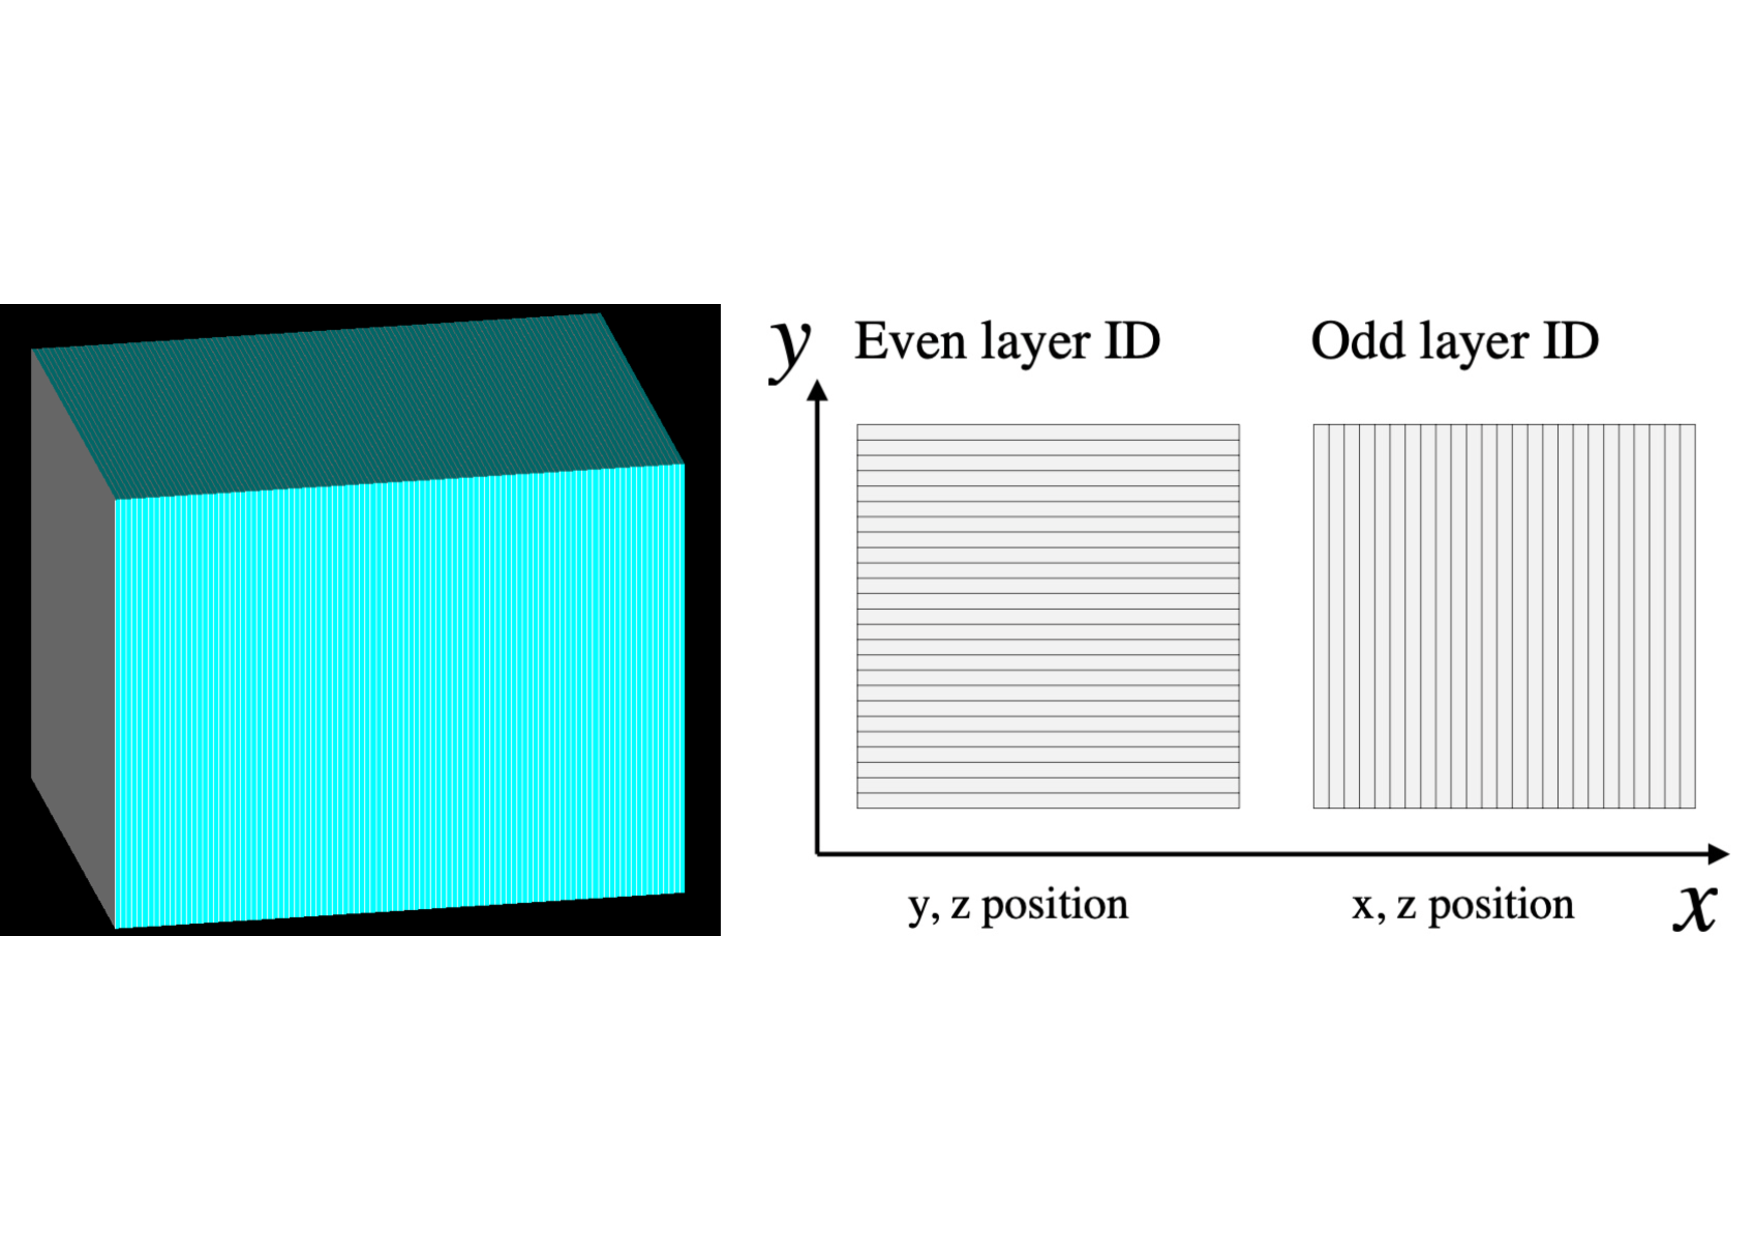
\includegraphics[width=0.85\textwidth]{figures/Sec2/Prototype_samplingcal.pdf}

%\caption{ The first trial of detector setup for simulation study on angle measurement. It is a sampling calorimeter consisting of alternating lead sheets and strips of plastic scintillator. }
%\label{fig:det_conf}
%\end{figure}

%\subsection{Electromagnetic shower Generation}
%\subsection{Properties of electromagnetic shower (EM shower)}
%We generated the EM shower generated inside the detector with GEANT4, which provides reliable results for them polish-up later).


%\subsection{Properties of electromagnetic shower (EM shower)}

%In general, the less the photon shower develops in the transverse direction, the more separable the photon clusters, and the higher the visible ratio, the better the energy resolution. However, these properties are incompatible as they have strong inverse correlation. For the trade-off configuration, we investigated the Molière radius and the visible ratio with several configurations. 

% 어떤 configuration, energy? 등등
% 2.5, 5, 10, 15, 20 mm for scint., 0.5, 1, 2 mm for lead 1GeV gamma
% For energy resolution, 100 MeV step 100MeV ~ 2GeV gamma


%\subsection{Backsplash}
% backsplash particle이 veto signal을 만들어 accidental event loss를 만든다.
% incident photon의 에너지와 각도를 바꿔가며 front surface로 빠져나오는 backsplash particle의 개수를 카운팅
% 1개 이상의 backsplash particle이 있으면 veto에 counting

%\subsection{XGBOOST: A toolkit for machine learning}
%\label{sec:anaML}
%Among many packages for machine learning in the high energy physics area~\cite{ATLAS:2020iwa}, we used the $\XGB$, supporting a scalable tree boosting system~\cite{xgboost:2016}. The $\XGB$ package is used to reconstruct the incident angle of incident $\gamma$ particles with deposit energies in the each channel, where secondary particles of the EM shower raise signals. Input data for the $\XGB$ are deposit energies for whole channels including zero-energies to tally with the requirement that the number of input data should be identical. For the $\XGB$ to reconstruct the angle, the training procedure for the $\XGB$ needs to be preceded. The training procedure helps the $\XGB$ study how $\gamma$ interacts with the detector and deposits the energy to the each channel with respect to the incident angle for a given $\gamma$ energy. Simulations are done with the uniform incident polar angle ($\theta$) distribution from 0 to 50 degree and the uniform azimuthal angle ($\varphi$) from 0 to 360 degree for the training, which makes the $\XGB$ possible to reconstruct events having 0~$<\theta<$~50~degree and 0~$<\varphi<$~360~degree. The reconstruction of $\theta$ by the $\XGB$, completing the training procedure, is tested with the fixed $\theta$ and uniform $\varphi$ from 0 to 360 degree.

\section{ANGLE RECONSTRUCTION}
\label{sec:res}

The incident angle of the $\gamma$ can be estimated as a results of machine learning by using the $\XGB$, which is one of the popular packages supporting a scalable tree boosting system~\cite{xgboost:2016}. We used energy deposits on each scintillator strips as input data for the $\XGB$, and the packages connects the relationship among the input data to estimate the incident angle. ** a little detail one or two senteces***

%are deposit energies on each scintillator strip by the generated shower particles. It includes the strips of zero-energy deposit in order to satisfy the requirement that the number of input data should be identical. As the training procedure, the $\XGB$ studies profiles of energy deposit to the individual strips with respect to the incident angle for a given $\gamma$ energy.  ({\it This part should be updated)}

For the training of the $\XGB$, we generated $\gamma$'s uniformly in the range 0 to 50 degrees of polar angle ($\theta$) and  0 to 360 degrees of azimuthal angle ($\varphi$) for given energy (training sample). By using another data set (testing sample) which was generated at a fixed polar angle, we estimated performance of angular reconstruction of the detector. The number of generated $\gamma$ was
$2\times10^5$ for the training sample and $1\times10^5$ for the testing sample, respectively.

%\subsection{Machine learning configuration}
%The configuration of the $\XGB$ can be organized with five parameters, described in Tab.~\ref{tab:XgbPar}. The parameters are selected as one providing better angular resolution. It is found that the Max. depth mostly affects the angular resolution, and the resolution is not enhanced for Max. depth~$>$~15 any more. It is also worth mentioning that configurations with N\_estimators larger than 1000 do not provide better resolution with the Max. depth~=~15. The angular resolution of the reconstruction is defined as the standard deviation of Gaussian function, whose parameters are evaluated by fitting the reconstructed angle distribution. Figure~\ref{fig:angle_reco_def} shows the reconstructed $\theta$ distribution with respect to each incident $\theta$ with described training parameters. The angular resolution for all $\theta$ is estimated to be 1.3~degree.

%\begin{figure}[!hbt]
%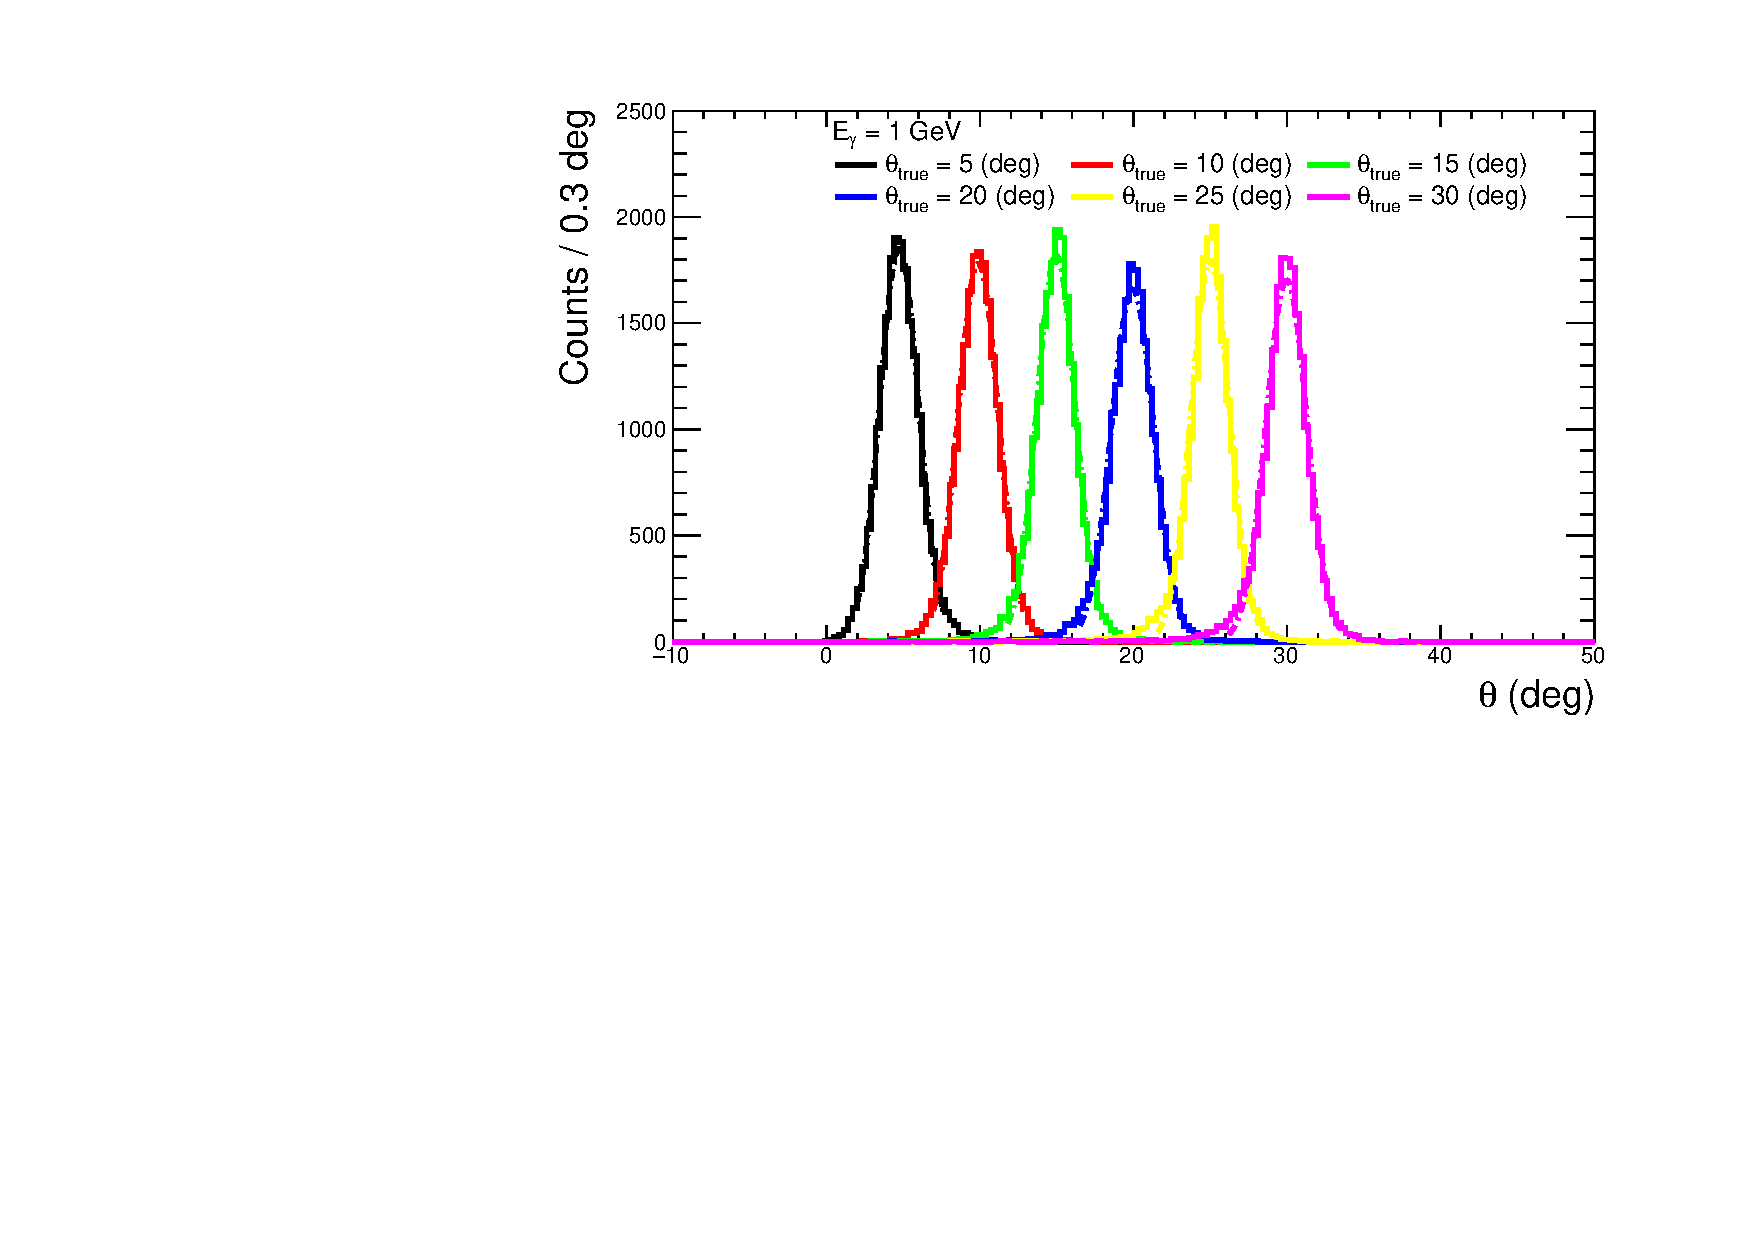
\includegraphics[width=0.89\textwidth]{figures/Fig1_reco_def.pdf}
%\caption{ (Color online) Reconstructed $\theta$ with respect to each true incident $\theta$ dotted lines denote each Gaussian function fitting the reconstructed $\theta$ distribution. The standard deviation of all Gaussian functions are estimated to be 1.3 degree.}
%\label{fig:angle_reco_def}
%\end{figure}

%\begin{table}[hbt!]
%\centering
%\caption{Parameterization of the $\XGB$}
%\begin{tabular}{cccc}
%\hline 
%Parameter & Function & Default value & Used value \\ \hline 
%N\_estimators & The number of decision trees & N.A. & 1000 \\  
%Max. depth & Possible maximum depth of tree structure & 6 & 15 \\ 
%Subsample & Fraction of total data used for a single decision & 1 & 1 \\ 
%Learning rate & Step length for calculation & 0.3 & 0.08 \\ 
%Gamma & Requirement on minimum loss function & 0 & 0 \\ 
%\hline
%\end{tabular}
%\label{tab:XgbPar}
%\end{table}

%\subsection{Detector dimension}
%\subsection{Angle reconstruction using Machine Learning}

%With the results of the $\XGB$ by using the training sample generated with the uniform distributions in both of polar and azimuthal angles, we estimated the incident angle of photons generated with a fixed value for a given energy. 
Figure~\ref{fig:angle_10degree} shows the distribution of reconstructed angles for 1-GeV $\gamma$ entered detector with 10 degrees of incident angle. %The Gaussian distribution (black solid line) provides the proper mean value,  the $\XGB$ can provide correct answer. 
We can get proper mean value of the distribution, however, it has heavier tail compared to that of the Gaussian distribution. In order to describe the obtained result more correctly, we tried to fit it with the Generalized Gaussian (GG) function. 

\begin{figure}[!hbt]
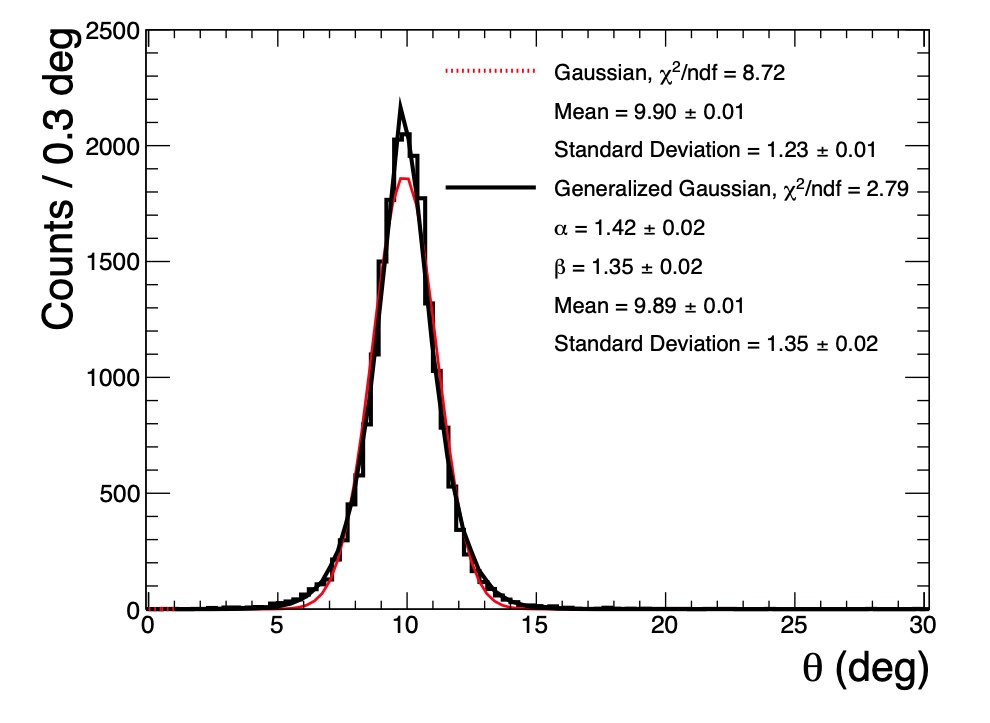
\includegraphics[width=0.7\textwidth]{figures/GG_fit.jpg}
\caption{ (Color online) Reconstructed $\theta$ with respect to 10 degrees of incident $\theta$. The gaussian function can not describe the tail region (red dotted line). The generalized gaussian function (black solid line) shows much better agreement with the obtained result.}
\label{fig:angle_10degree}
\end{figure}

%In order to include the heavier tail more correctly in the performance study, we tried to fit the distribution with two different function; one is a convolution of a Lorentz and Gaussian distribution (Voigt function) and the other is a Generalized Gaussian function.
%The Voigt fuction expressed as 
%\begin{equation}
%V(x; \sigma, \gamma) = \int_{- \infty}^{\infty} G(x';\sigma)L(x-x';\gamma) dx',
%\end{equation}
%becomes to be Lorentz distribution $L(x; \gamma)$ in case of $\gamma$=0 
%\begin{equation}
%L(x;\mu, \gamma) = {\gamma \over {\pi ((x-\mu)^2 + \gamma^2)}}
%\end{equation}
%of peak position at x=$\mu$ in case of $\sigma$ =0 
%and to be Gaussian distribution $G(x;\sigma)$
%\begin{equation}
%G(x;\mu, \sigma) = {1 \over {\sqrt{2 \pi} \sigma}} e^{-(x-\mu)^2/2\sigma^2} 
%\end{equation}
%when the $\gamma$ equal to be zero. The function is available in the analysis framework of the ROOT~\cite{Voigt}, and  improves the fitness a little. 

The GG function provides more flexible modeling to data than the Gaussian can do by introducing an additional parameter to describe the shape of distribution. This function was suggested by Subbotin~\cite{Subbotin} in 1923 treating the accidental errors not only to be continuous but also to be expanded in the power series. Its probability density function is expressed as 
%has received considerable attention especially at the image processing studies\cite{Dytso},  
%Among various parametrization of the function, we take that its probability density distribution (pdd) is given as~\cite{Gonzalez}  
\begin{equation}    
  % GG(x;\mu, \sigma,     p) = {C_p \over \sigma} e^{-{|x-\mu|^p}/{2 \sigma ^p}}, 
   %f(x; \mu, \alpha, \beta) = {\beta \over {2 \alpha \Gamma(1/\beta)}} e^{-(|x-\mu|/\alpha)^\beta} , 
     f(x; \mu, \alpha, \beta) = \frac{\beta}{2 \alpha \Gamma(1/\beta)} e^{-(|x-\mu|/\alpha)^\beta} , 
%   f(x; \mu, \alpha, \beta) = {\beta \over {2 \alpha \Gamma (1/\beta)}} e^{-(|x-\mu|/\alpha)^\beta} , 
\end{equation}    
where $\beta$ is the so-called shaping factor
%Also  
%\begin{equation}    
%    A ={ {\beta p}  \over {2\Gamma(1/p)}},
%\end{equation}
and the $\Gamma(.)$ is the gamma function.
It becomes the Laplace distribution if $\beta$=1 
\begin{equation}
LP(x;\mu, \sigma) = \frac{1}{\sqrt{2}\sigma} e^{-{\sqrt{2}{|x-\mu|} / \sigma}} 
\end{equation}
and Gaussian distribution
\begin{equation}
G(x;\mu, \sigma) = \frac{1}{\sqrt{2 \pi} \sigma} e^{-(x-\mu)^2/2\sigma^2} 
\end{equation}
for $\beta$=2.  The second moment of the GG function is given as
\begin{equation}    
    E[X]^2  = \alpha^2 \frac{\Gamma(3/p)}{\Gamma(1/p)}  \equiv \sigma^2 , 
\end{equation}
which becomes the variance of the Gaussian distribution in case of the $\beta$=2. This value can be interpreted equal footing regardless of the $\beta$-values, and will be used as the angular resolution for given detector configuration from now.
%we can treat it as a width of the distribution which contains same meaning %regardless of the p-values.  


\begin{figure}[!hbt]
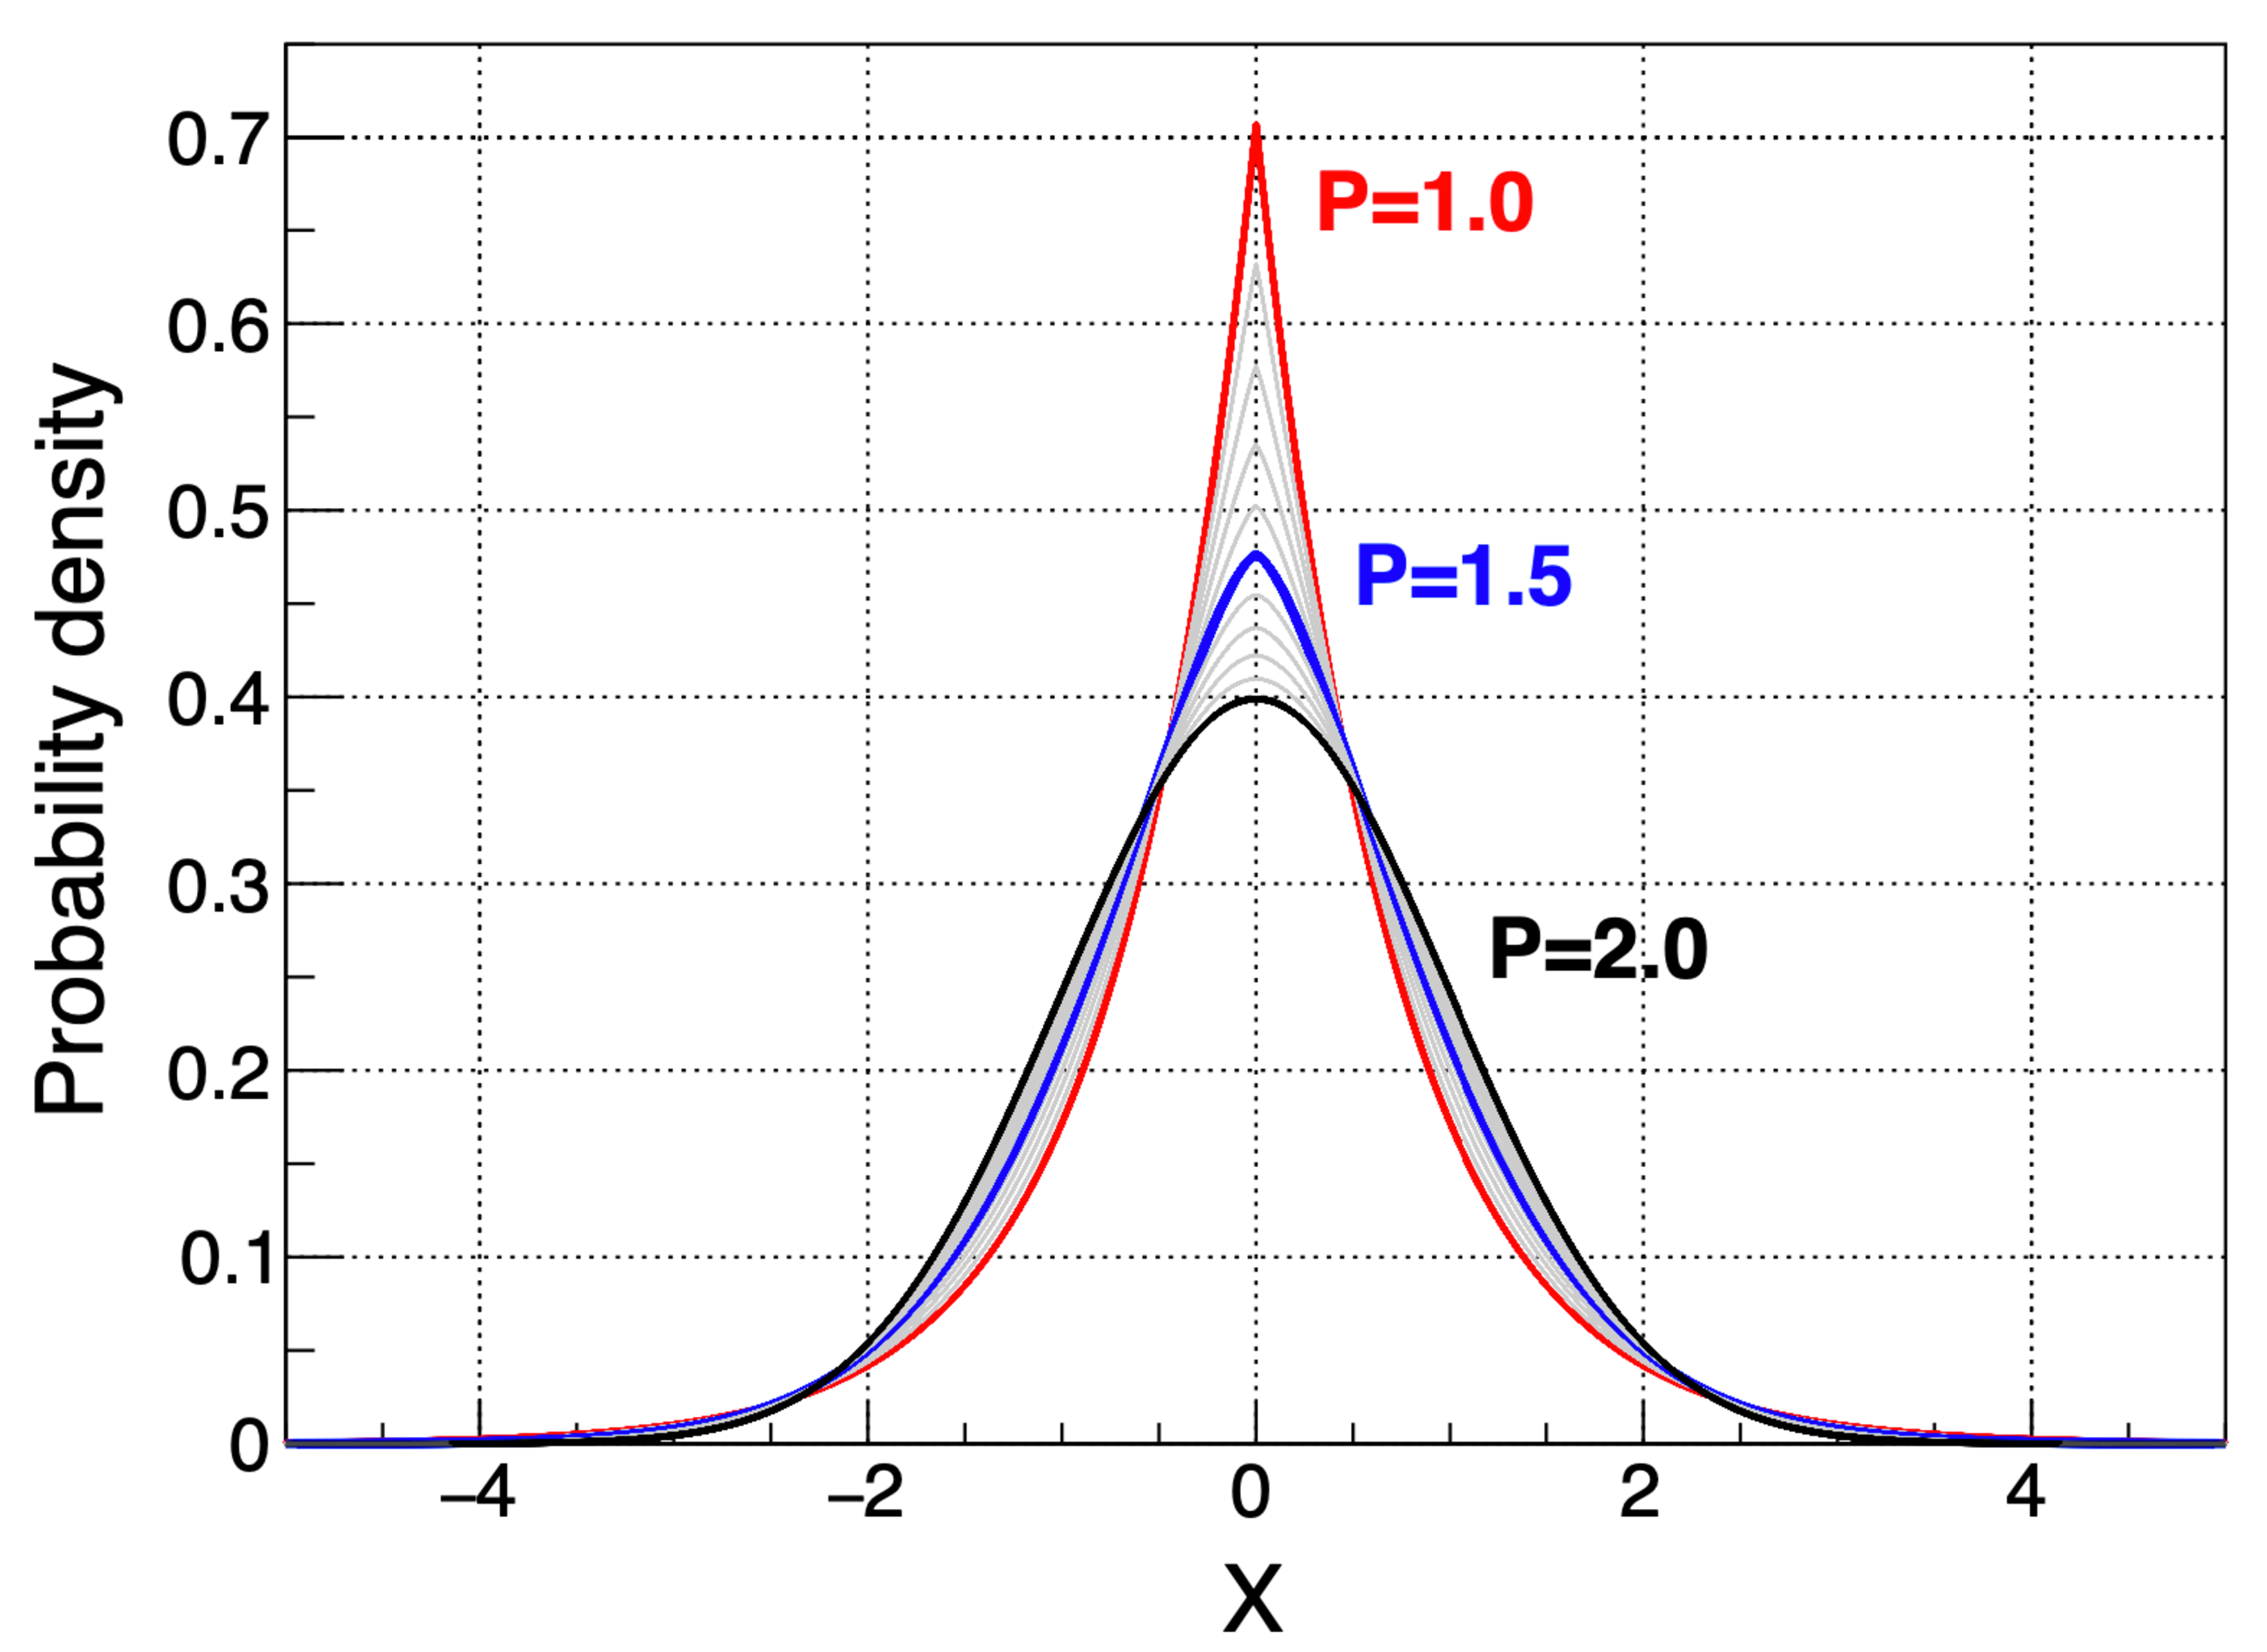
\includegraphics[width=0.45\textwidth]{figures/PDF_Gonzalez.pdf}
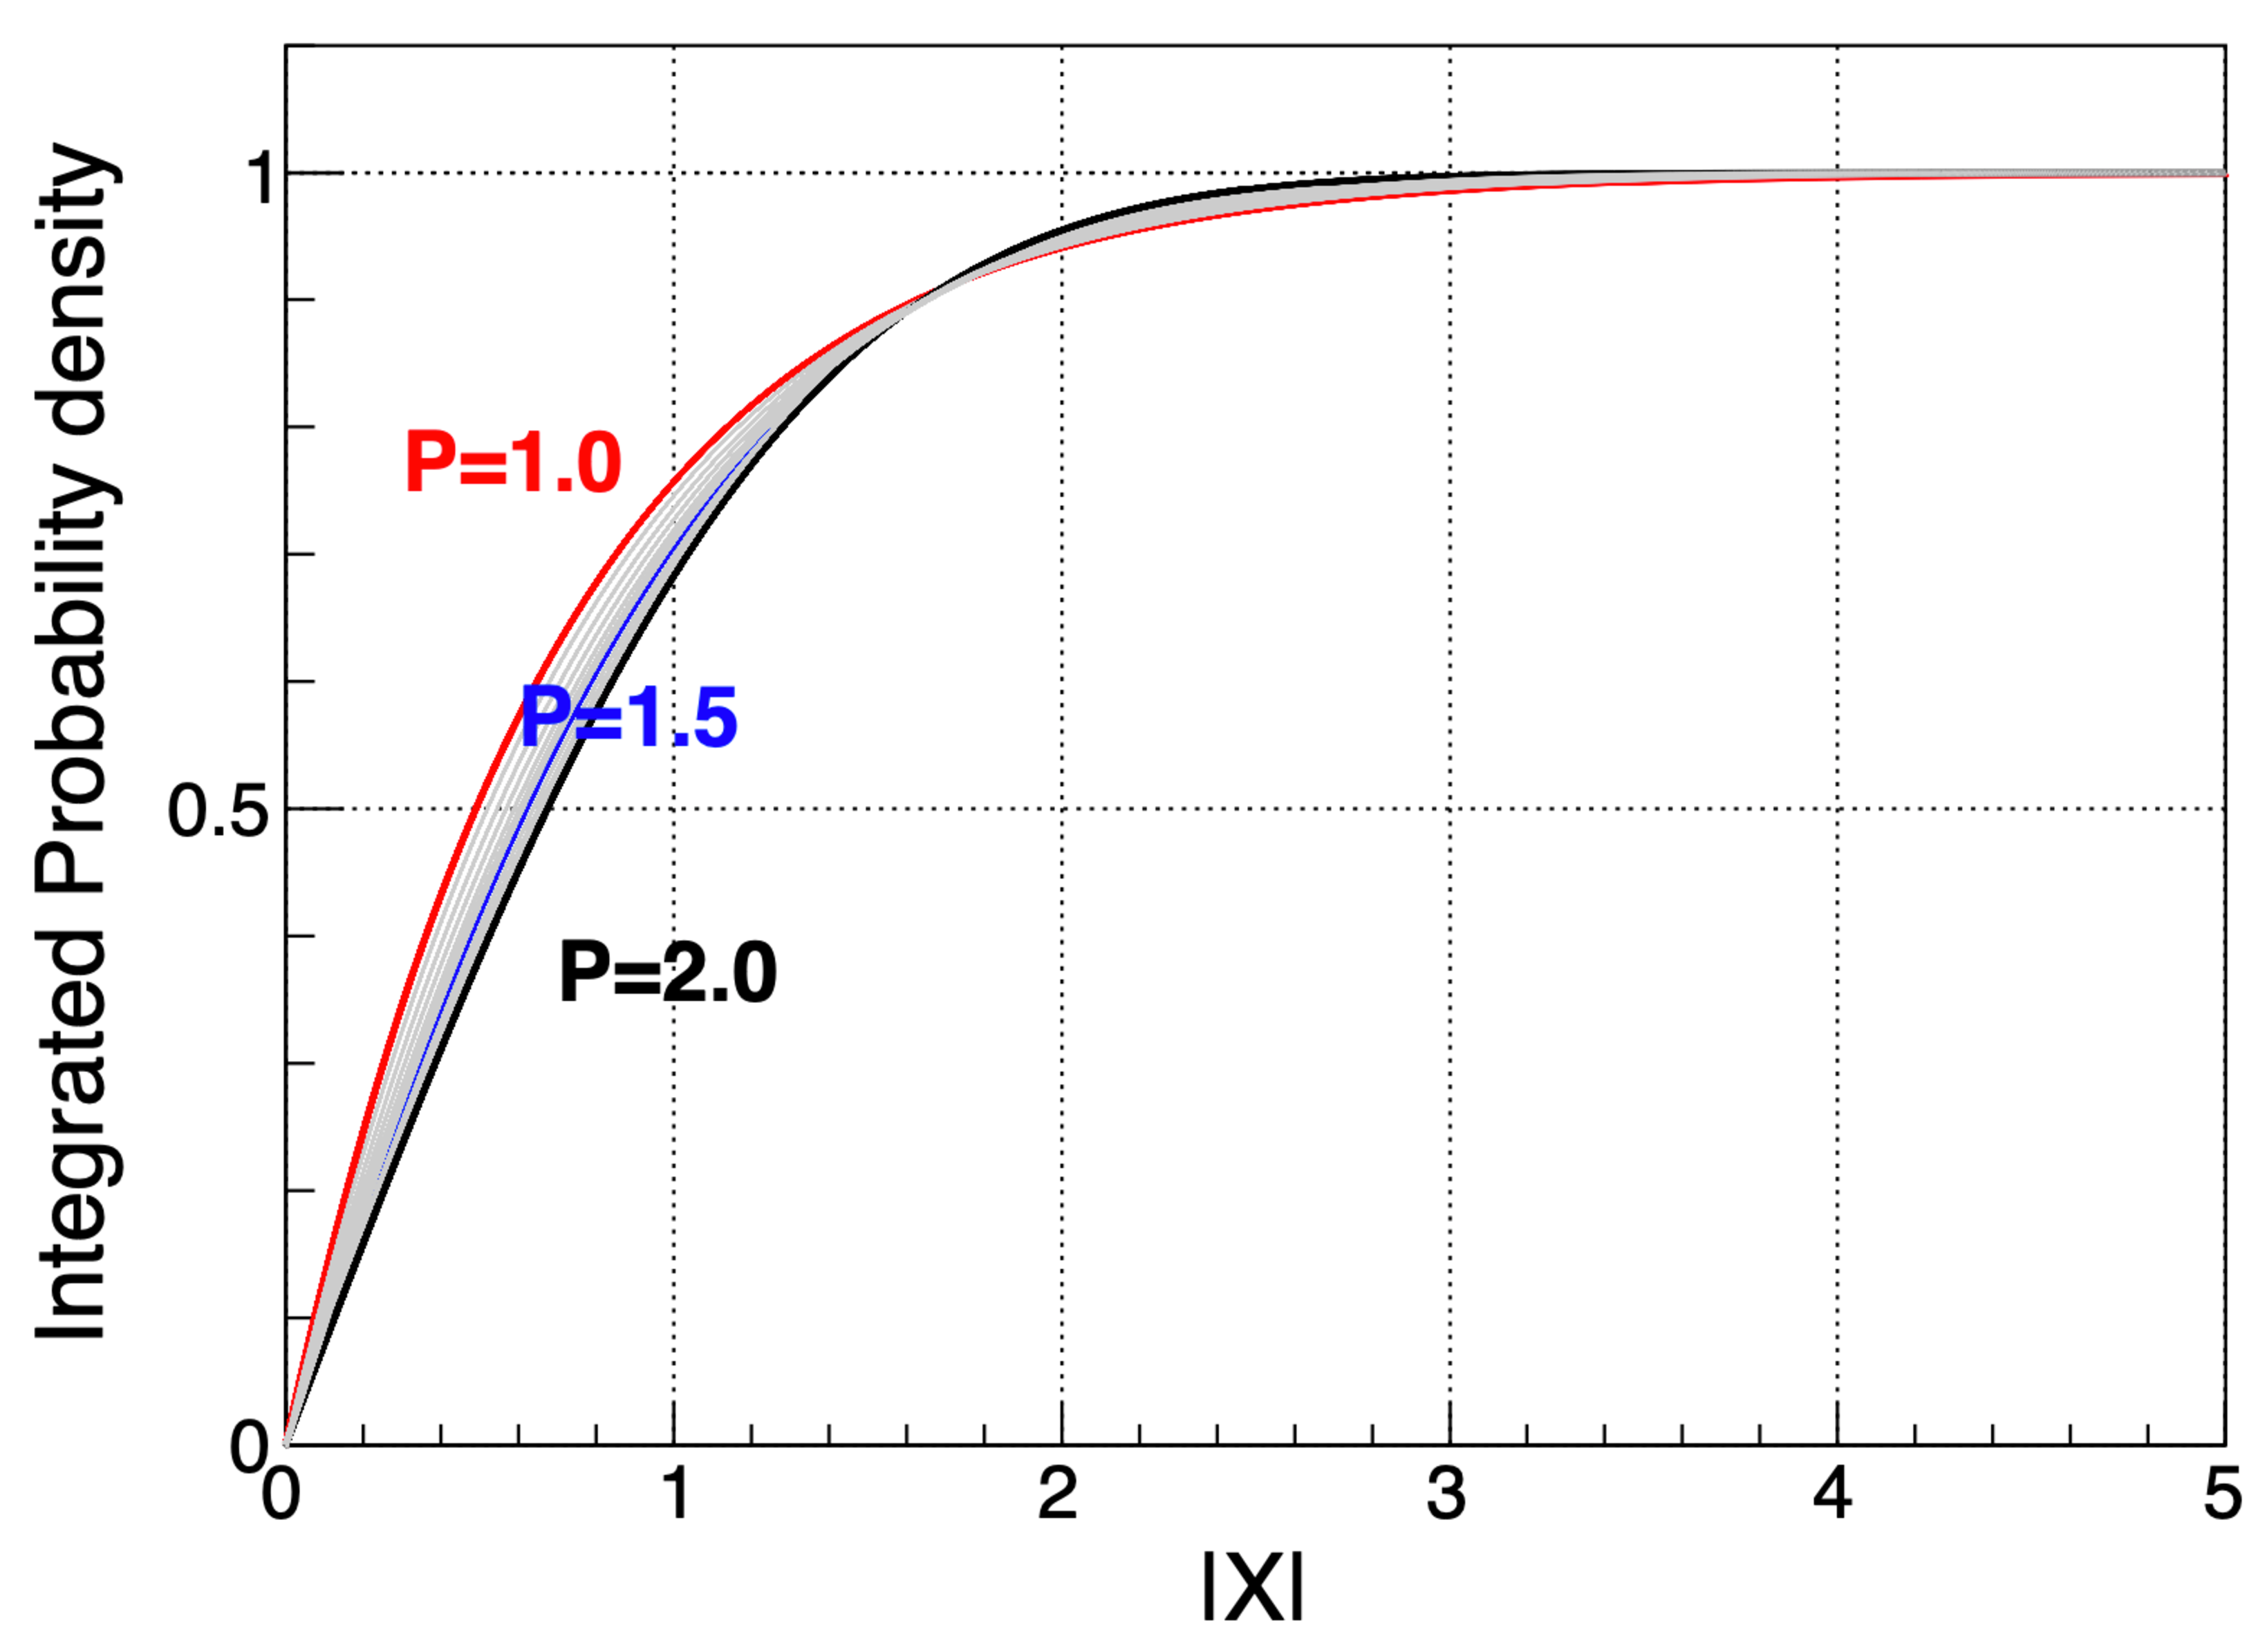
\includegraphics[width=0.45\textwidth]{figures/Int_Gonzalez.pdf}
\caption{ The probability density distribution (left), and their integrated distributions (right) of the generalized gaussian (GG) function in the case of  $\mu = 0$ and $E[X]^2 = 1$ for various shaping paramete $\beta$. It changes from the Laplace ($\beta$=1) to the Gaussian ($\beta$=2) distribution according to the $\beta$. On the other hands, their integral probability density show similar distributions implying its second moment can be interpreted equally regardless of the $\beta$ values in the range of $1<\beta<2$.}
\label{fig:GG_pdf}
\end{figure}

Figure~\ref{fig:GG_pdf} (left) shows the probability density distribution of the GG function in the case of $\mu = 0$ and $E[X]^2 = 1$ for different $\beta$ values from 1 to 2. We can figure out the change from the Laplace ($\beta = 1$) to the Gaussian distribution ($\beta=2$). As shown in the right plot of the Fig.~\ref{fig:GG_pdf}, the integrated probability for 1$\sigma$ interval becomes to be from 68.3$\%$ ($\beta=2$) to 75.7$\%$ ($\beta=1$). In the case of $\beta=1.5$ as obtained from the data fitting, it is to be 71.2$\%$ which is just 4$\%$ larger than that of the Gaussian. Moreover, a statement of "1.7$\sigma$ interval contains 91$\%$ of entries" can be applied in range of $1<\beta<2$, thus we will use the $\sigma$ as a definition of the angular resolution in this paper.    
%When we take an angular resolution as the width of fitted distribution, it is determined by the two parameters, $\sigma$ and p. Figure~\ref{fig:GG_pdf} shows distributions of probability density (left) and integrated the density for $\sigma =1$ with changing value of p from 1.0 to 2.0. We can parameterize the angular resolution, $\sigma_{R}$ as
%\begin{equation}
%\sigma_{R} = f(p) \cdot \sigma,
%\end{equation}
%where the $f(p)$ is a empirically determined scale factor from the Fig.~\ref{fig:GG_pdf} (right). With the definition, the integrated probability becomes 68.3$\%$ inside the $\sigma_R$ for all p values in the range of $1 \leq p \leq 2$.

%for a given value of p in the range of. That is, the fitted result of the Fig.~\ref{fig:angle_10degree} ($\sigma$=

%its performance of the angle measurement is tested with the test sample forq given angle.
%tested its reconstruction performance with $10^6$ gamma samples for each fixed polar angle from $\theta=$ 5 to $\theta=$ 30 in 5 degrees steps.
%of the $\XGB$ by using $10^6$ gamma samples generated with uniform distribution in both of polar angle in range of 0 to 50 degrees and azimuthal angle of 0 to 360 degrees, we tested its reconstruction performance with $10^6$ gamma samples for each fixed polar angle from $\theta=$ 5 to $\theta=$ 30 in 5 degrees steps. 
%Figure~\ref{fig:angle_reco_def} shows the distribution of reconstructed angles for incident gammas those have 1-GeV of energy and 10-degree of polar angle. The distribution has heavier tail compared with that of the Gaussian, and we tried to fit the distribution with the Generalized Gaussian distribution. The distribution  

%which agree well with the generated values.
%The angles are properly reconstructed with a typical resolution as 1.2 degrees. There are no significant differences among the various incident angles. 
%Typical angular resolution is obtained as 1.2 degrees and does not show significant dependency on incident angle.



\begin{figure}[!hbt]
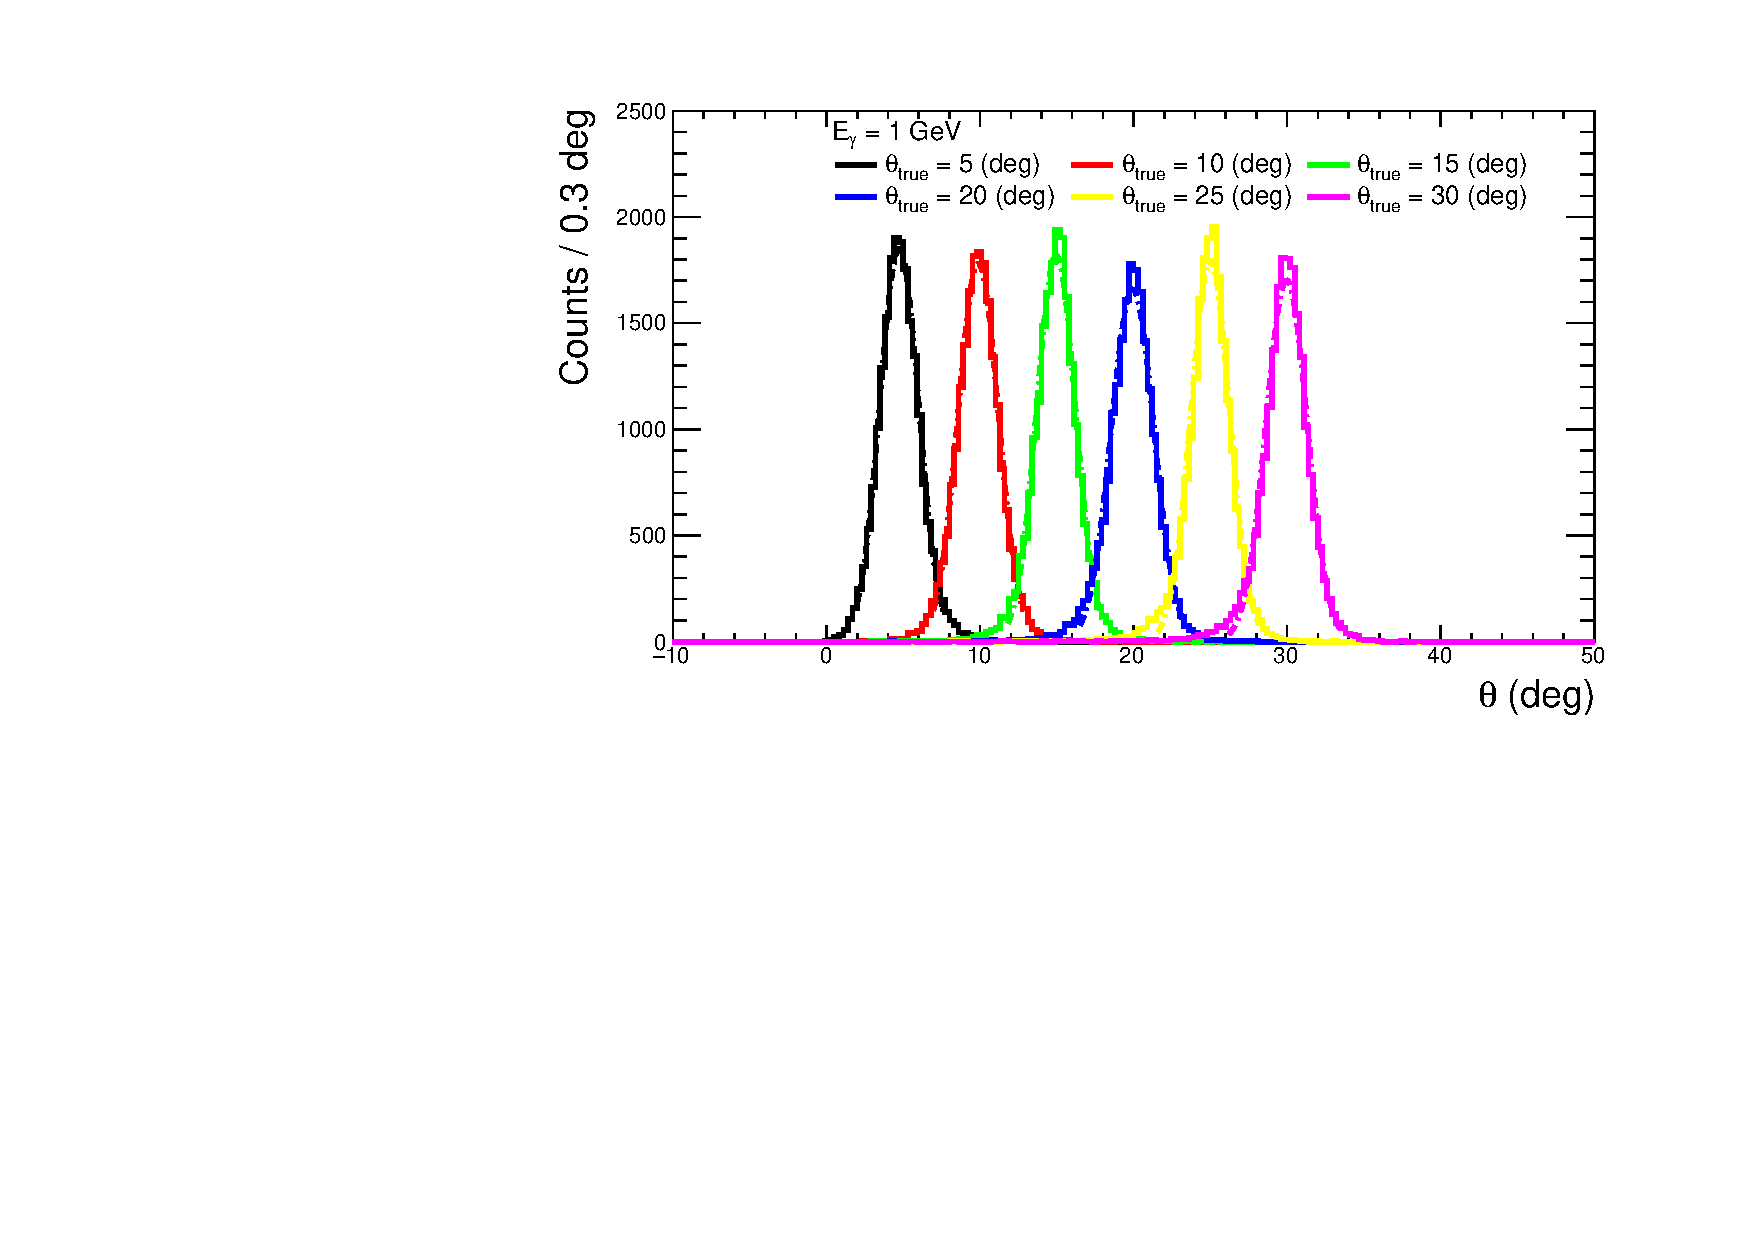
\includegraphics[width=0.89\textwidth]{figures/Fig1_reco_def.pdf}
\caption{\textcolor{red}{plots should be updated}
Angular resolution for different incident angles (left) and shape parameter $\beta$ of reconstructed angluar distribution (right).}
\label{fig:angle_reco_def}
\end{figure}

Since the angular resolution depends on the hyperparameters of the $\XGB$ which control the details of the training process, we scanned them with monitoring the angular resolution $\sigma$ defined at the Eq. 7. There are five hyper parameters which can be optimized by user, and correlated among them. Figure~\ref{fig:par_scan} shows part of the scanning results, which enables us to determine the best parameters set to provide the best angular resolution. 
%their values are selected to provide the best angular resolution as described in
The decided values of the parameters are given in Table~\ref{tab:XgbPar} with their function in the training process. %Among the parameters, the Max. depth rapidly improves the angular resolution with increasing its value until 15. The N\_estimators also improves the angular resolution with increasing its number, which is correlated to the value of the Max. depth. Its optimal condition becomes 1000 when the Max. depth is 15. ({\it This part should be updated) - can we mention more detail?}
 
\begin{figure}[!hbt]
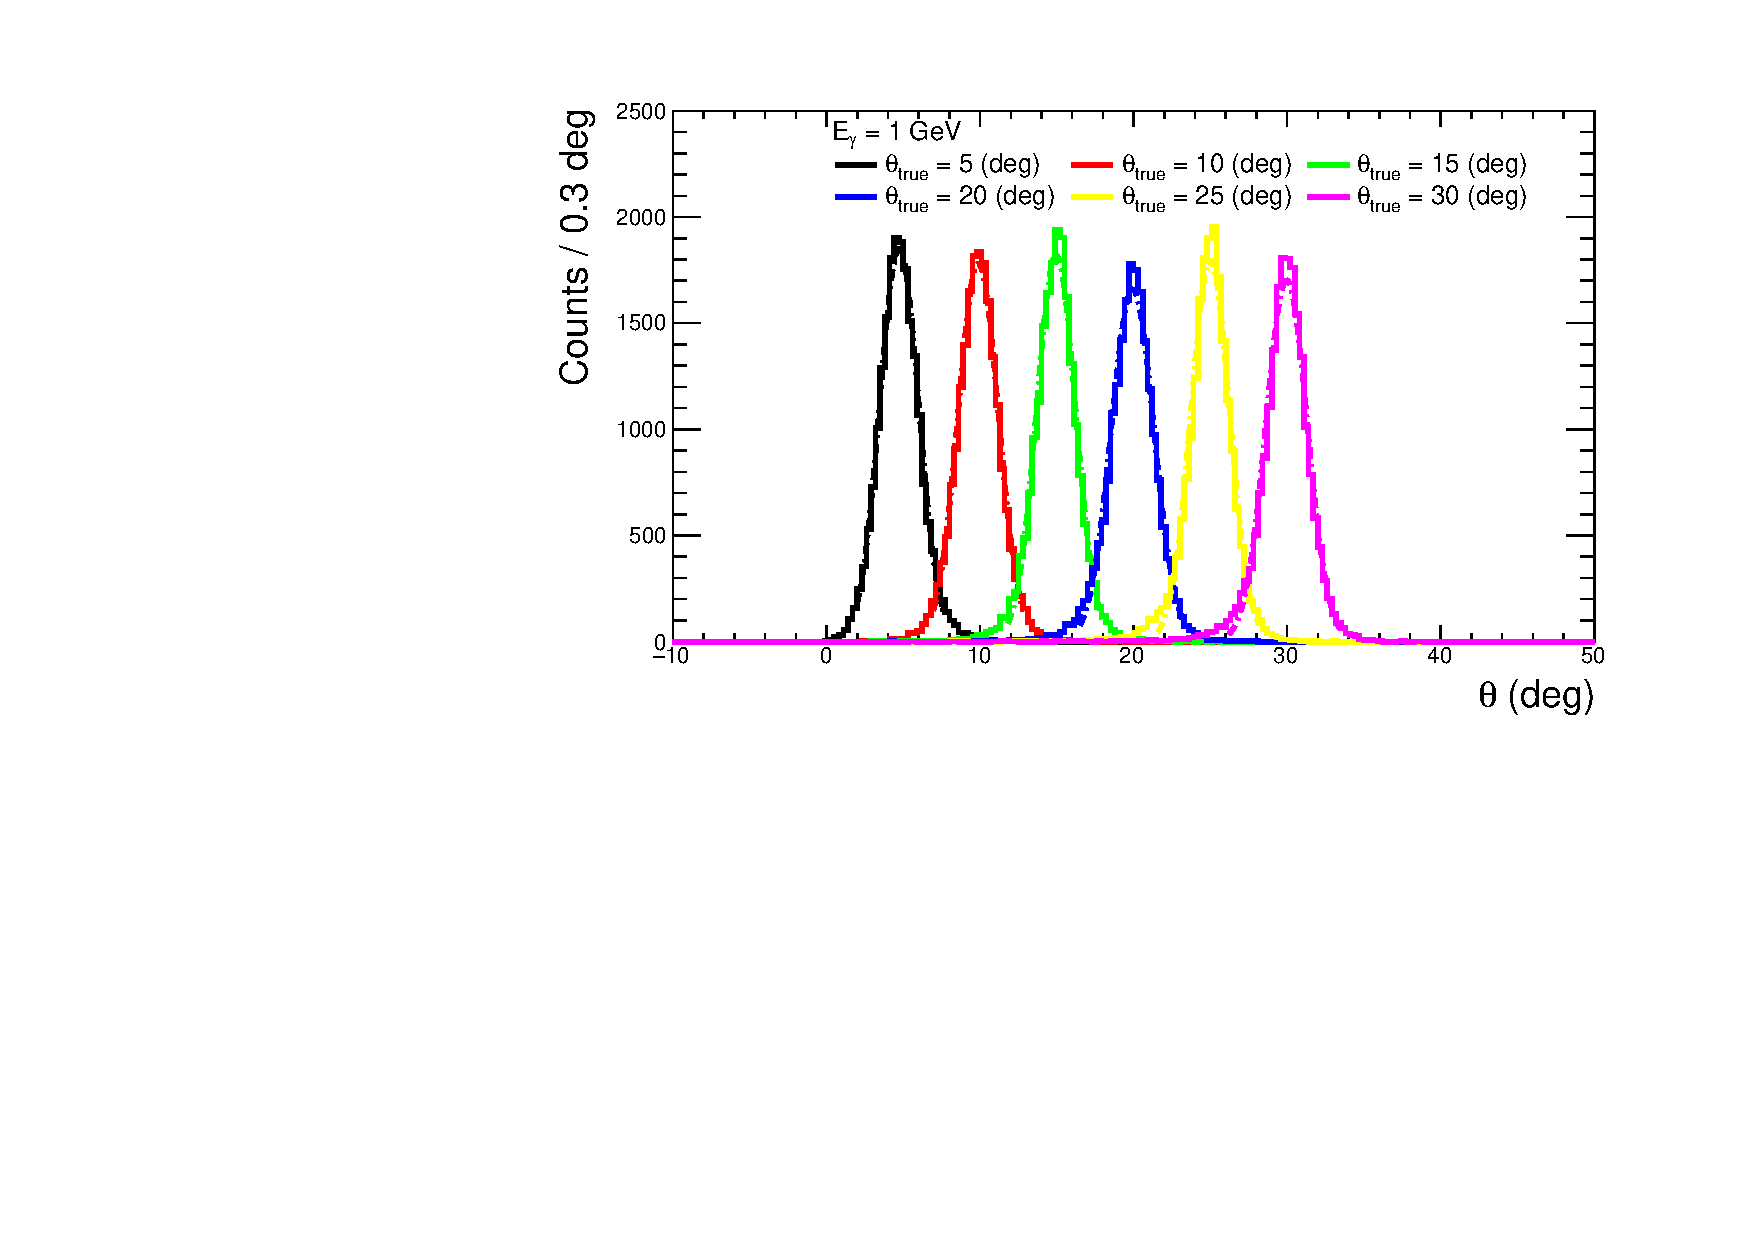
\includegraphics[width=0.89\textwidth]{figures/Fig1_reco_def.pdf}
\caption{\textcolor{red}{plots should be updated}
Angular resolution for different hyperparameter valuse.}
\label{fig:par_scan}
\end{figure}

%performance of the angular reconstruction is tested with independently generated data samples with fixed $\theta$ and uniform $\varphi$ from 0 to 360 degrees. ({\it This part should be updated)}

\begin{table}[hbt!]
\centering
\caption{Hyperparameters of the $\XGB$}
\begin{tabular}{cccc}
\hline 
Parameter & Function & Default value & Used value \\ \hline 
N\_estimators & The number of decision trees & N.A. & 1000 \\  
Max. depth & Possible maximum depth of tree structure & 6 & 15 \\ 
Subsample & Fraction of total data used for a single decision & 1 & 1 \\ 
Learning rate & Step length for calculation & 0.3 & 0.08 \\ 
Gamma & Requirement on minimum loss function & 0 & 0 \\ 
\hline
\end{tabular}
\label{tab:XgbPar}
\end{table}


\begin{figure}[!hbt]
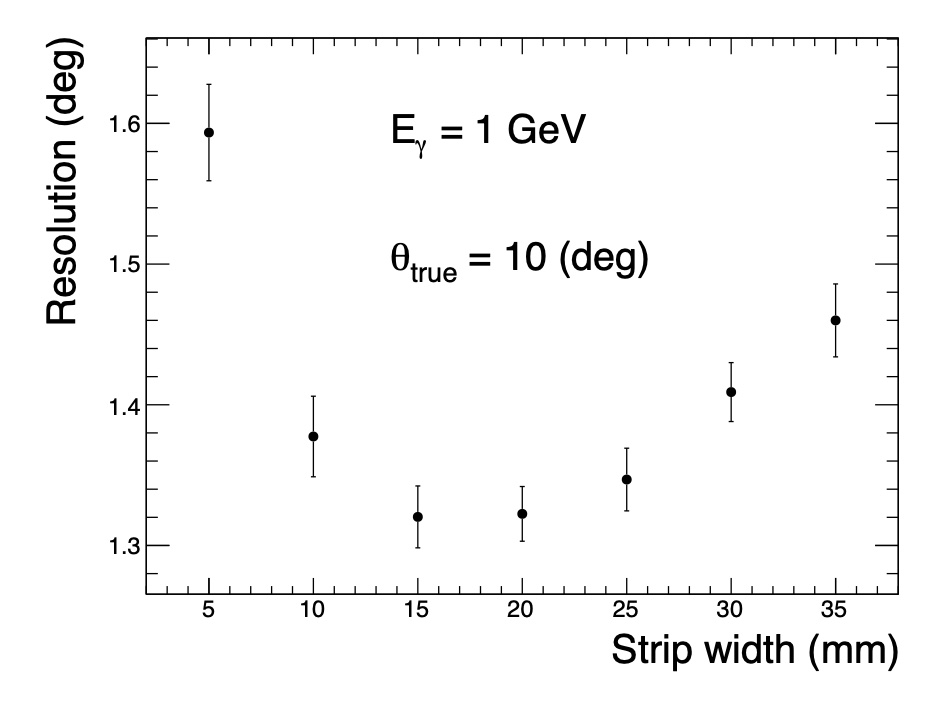
\includegraphics[width=0.58\textwidth]{figures/res_width.jpg}
\caption{ The angular resolution as a function of the scintillator strip width for 1 GeV $\gamma$. The incident angle for each simulation is fixed as 10 degree.  }
\label{fig:angle_reco_width}
\end{figure}

For the study of the angle-reconstruction performance for different incident angles, we generated test samples of fixed value in range of 5 to 45 degrees with 5-degree steps. Each test sample contains $10^5$ $\gamma$'s and common parameter settings are used for calculating their incident angle, which showed similar performance for all samples. Figure~\ref{fig:angle_reco_def} shows the angular resolutions defined in Eq. 7 for each incident angle (right) and shape-parameter $\beta$ (left).The performance of the angle reconstruction does not depend on the incident angle. 

%With the scintillator strips having a narrower width, we may get more precise information about the shower shape. 
With an assumption that getting more precise information on the shower profile enables us to estimate with better resolution, we have studied the angle reconstruction by changing the width of the strips from 5 mm to 35 mm in 5 mm steps. As shown in Fig.~\ref{fig:angle_reco_width}, the best resolution is obtained when the width is 15mm. We can interpret that the larger-width configurations suffer the dilution of shower information and produce worth result. On the other hands, the narrower-width configuration does insufficient training due to limited statistics because of increased input features. This problem will be explained detailed later. 


%In order to figure out the optimal detector configuration providing the best angular resolution, we repeated the calculation by changing the width of the strips from 5 mm to 35 mm in 5 mm steps. Even though the narrower width is expected to provide more precise information about the shower shape, it does not mean to provide the better resolution as shown in Fig.~\ref{fig:angle_reco_width}.  The angular resolution is not changed with increasing strip width up to 25 mm, which implies that the precise information on the shower shape is not essential to the angular resolution in a certain range because  of the stochastic nature of the shower generation. On the other hand, there is a possibility of insufficient training due to rapid increasing of the number of input according to the finer segmentation, while the number of events and hyper parameters for the training remain the same values optimized for the configuration of the 15-mm width.


%because the shower generation is a stochastic process and low energy photons produced by the Compton scattering and photoelectric effects are not aligned in the incident direction. 

%The main reason seems to be a limitation of the number of training sample caused by lack of computer memory. 
%As shown in Fig XXX, the obtained angular Aresolution for the 5-mm width is improved with increasing the number of training sample, while the other larger width is saturated already. %achine learning for increasing number of input data. XXXX. 
%Also, the angular resolution is not changed with increasing strip width up to 25 mm, which means the more precise information is not essential for the better angular resolution because the shower generation is a stochastic process and low energy photons produced by the Compton scattering and photoelectric effects are not aligned in the incident direction. 

%On the other hand, the finite size of the strip is related to the effect of incident gamma position. The previous results given in the Fig.~\ref{fig:angle_reco_width} are obtained from the data samples in which the incident gammas enter to a fixed position, the center of the strip. When we generated the gammas entering uniformly to the strip, we get the angular resolution as shown in Fig. xxx. Base on the results, we decide the width of the strip as xxx mm for a testing module to confirm the M.C. studies.
%The performance of the detector is tested with different detector dimensions. Different geometries are simulated in the Geant4 package and corresponding training procedures are applied with the same number of training events as 100,000. Figure~\ref{fig:angle_reco_width} shows the angular resolution of the reconstruction as a function of the scintillator strip width with 5-mm-wide steps. It if found that the configuration with 15-mm-wide strips provides better resolution than one with smaller strip widths, and configurations with larger strip size than 15 mm do not provide improved resolution so that the width of the strip is determined to be 15 mm.


\begin{figure}[!hbt]
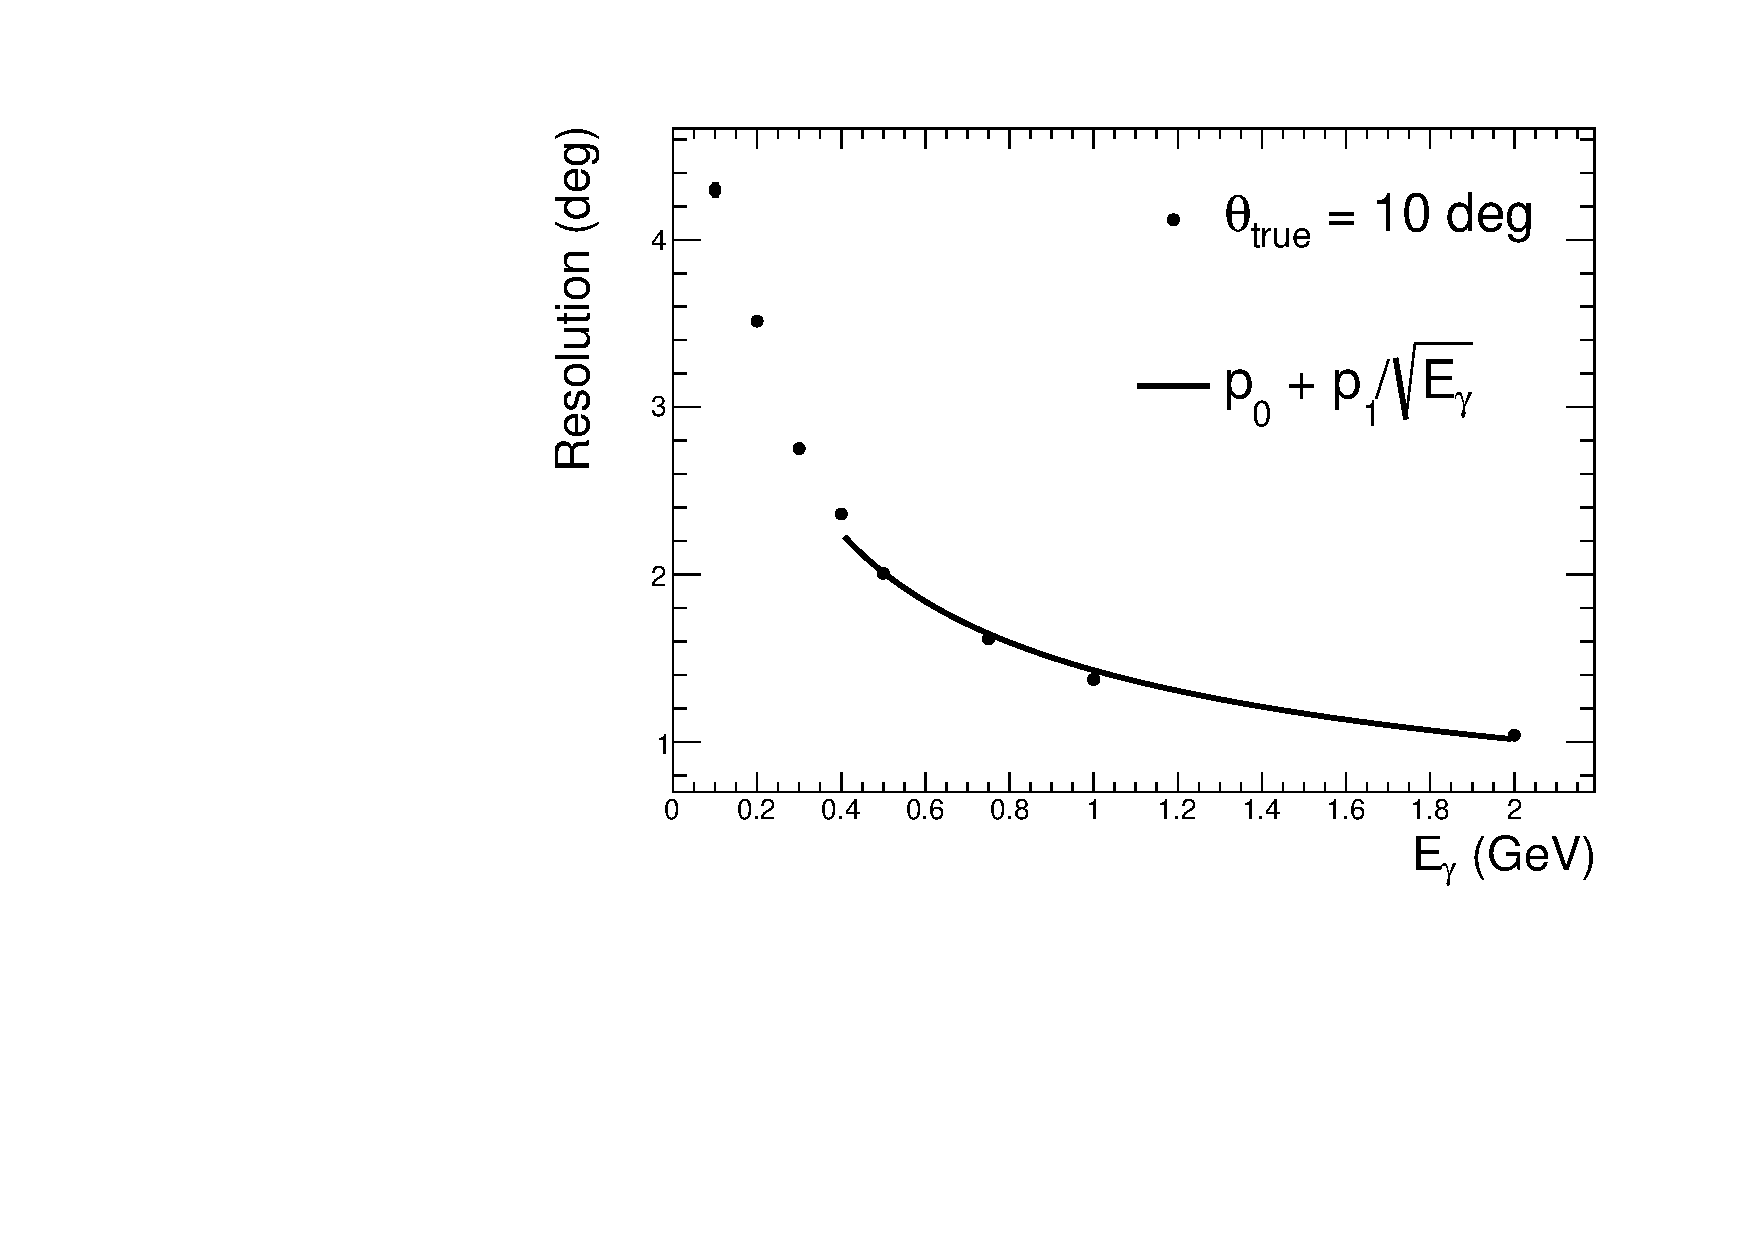
\includegraphics[width=0.48\textwidth]{figures/Fig5_reco_graph.pdf}
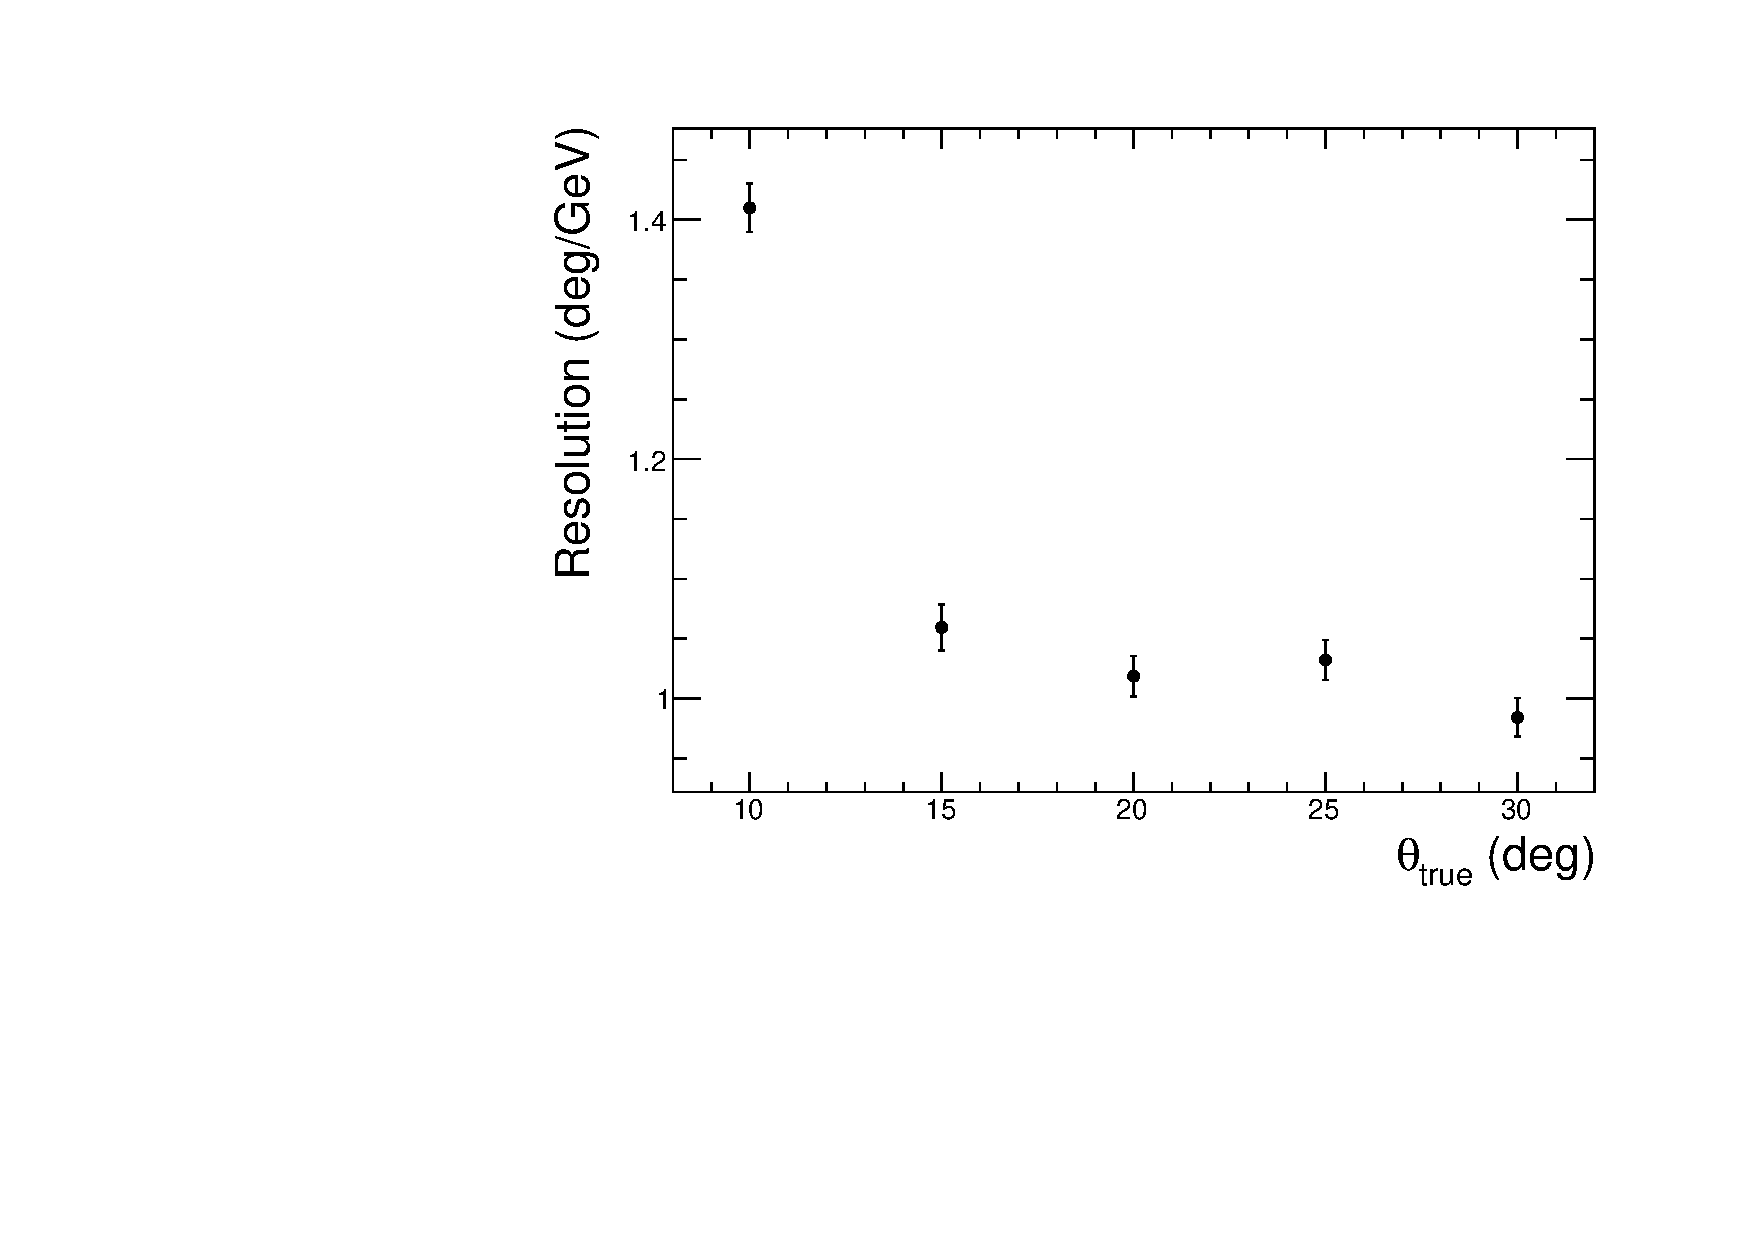
\includegraphics[width=0.48\textwidth]{figures/Fig5_reco_inc.pdf}
\caption{ The angular resolution as a function of $\gamma$ energy (left), and the angular resolution for 1 GeV as a function of incident $\theta_{\rm{true}}$ (right). }
\label{fig:angle_reco_dep_gr}
\end{figure}

Figure~\ref{fig:angle_reco_dep_gr} shows the angular resolution as a function of the incident $\gamma$ energy for $\theta_{\rm{true}}=$~10~degrees on the left panel. The resolution is fitted with $p_{0} + p_{1}/\sqrt{E_{\gamma}(GeV)}$, where the $p_{0}$ denotes the contribution from energy-independent term and \textcolor{blue}{is estimated to be zero ($<$= is this true ?)}, and the $p_{1}$ denotes the contribution from energy-dependent term, mainly related with the development of the EM shower. The estimated $p_{1}$ for different $\theta_{\rm{true}}$ can be seen in the right panel of fig.~\ref{fig:angle_reco_dep_gr}. They are deviating within $\pm$~0.05~deg range from the 1.25~deg.



\begin{figure}[!hbt]
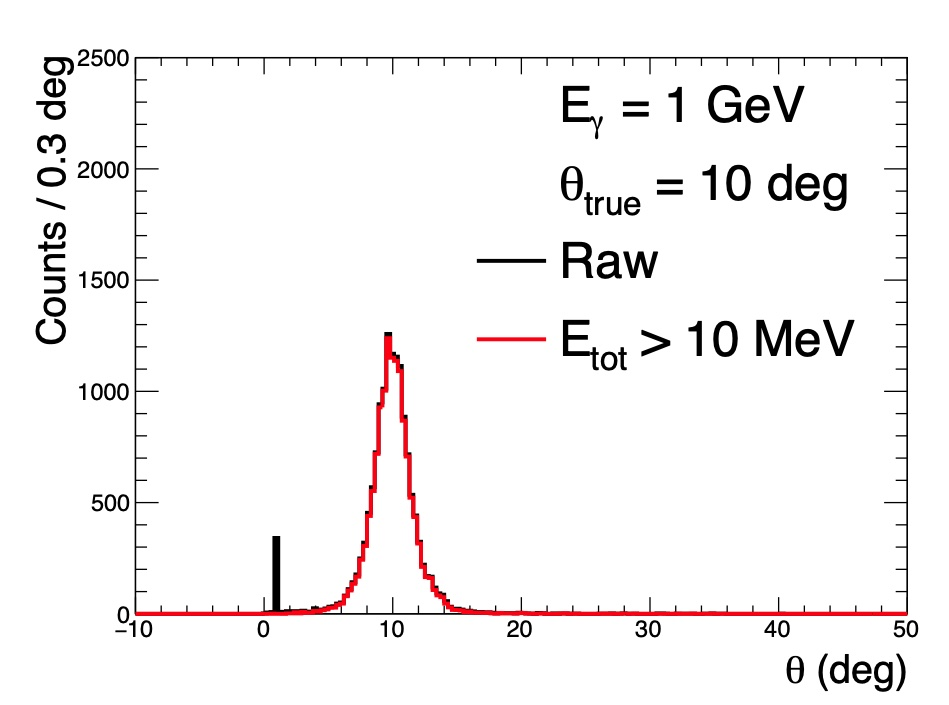
\includegraphics[width=0.48\textwidth]{figures/res_Nlayer.jpg}
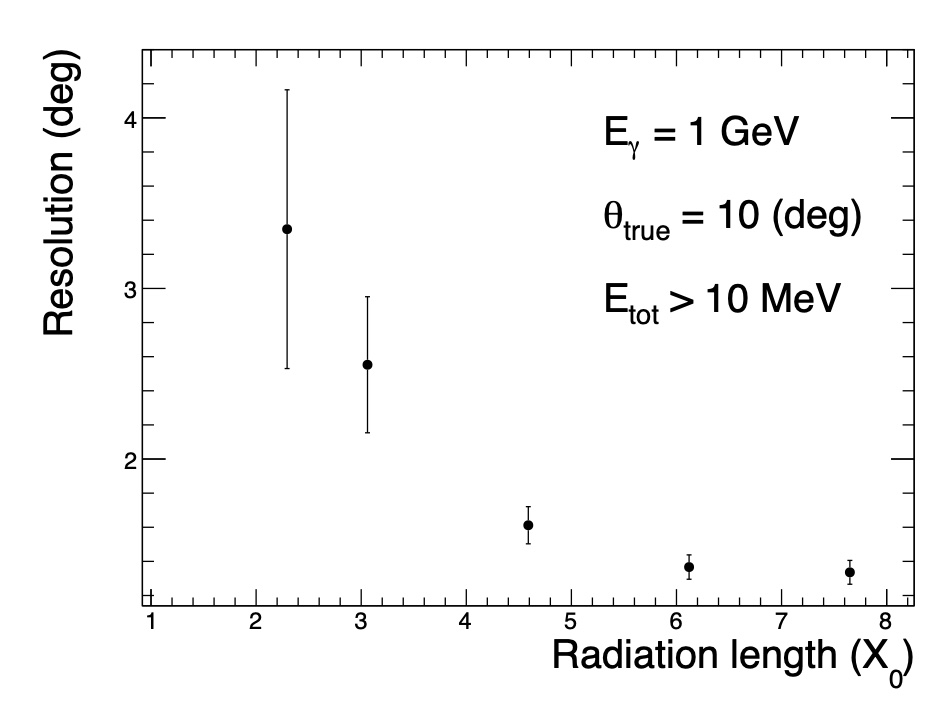
\includegraphics[width=0.48\textwidth]{figures/resol_Nlayer.jpg}
\caption{ (Color online) Reconstructed $\theta$ for 1 GeV and $\theta_{\rm{true}}=$~10~deg $\gamma$ with (red) and without (black) the total energy ($E_{\rm{tot}}$) selection (left), and the angular resolution as a function of front layer depth used for the reconstruction (right). The inefficiency for 4.6$X_{0}$ is estimated to be 5.8\% with 10 MeV selection criteria. The large error bars less than 4.6 Xo is due to insufficient fitting because the reconstructed angular distributions deviated from the General Gaussian function. }
\label{fig:angle_reco_layer}
\end{figure}

Considering a measurement of incident angle only, we don't need the full-scaled detector to contain the generated shower completely. We can expect 99\% of $\gamma$ will start to generate shower inside detector within 5 radiation length (Xo). The left panel of Figure~\ref{fig:angle_reco_layer} shows reconstructed angle by using only the front 24 layers of the detector which corresponds to the length of 4.6 Xo for 1 GeV $\gamma$. The failed events located near the 0 are due to insufficient energy deposit ($<$ 10 MeV) to reconstruct the angle, of which ratio is estimated to be 5.8\%. As shown in the right panel of Figure~\ref{fig:angle_reco_layer}, the 4.6 Xo is needed to achieve equivalent resolution to that of the full-scaled detector. This results suggest that we can design a calorimeter producing complete information of incident $\gamma$ for itself by putting an fine segmented sampling calorimeter in front of the main calorimeter.

The obtained angular resolution is determined by combined multiple sources, mainly the performance of learning process, number of layers for the measurement and the width of strips. Figure~\ref{fig:multi-parameter} shows the relation among the sources. For the larger width (25mm), the larger numbers of layers gives the better resolution (left). In order to achieve the best resolution for narrower width (5mm), we need much larger number of events for training the $\XGB$  


\begin{figure}[!hbt]
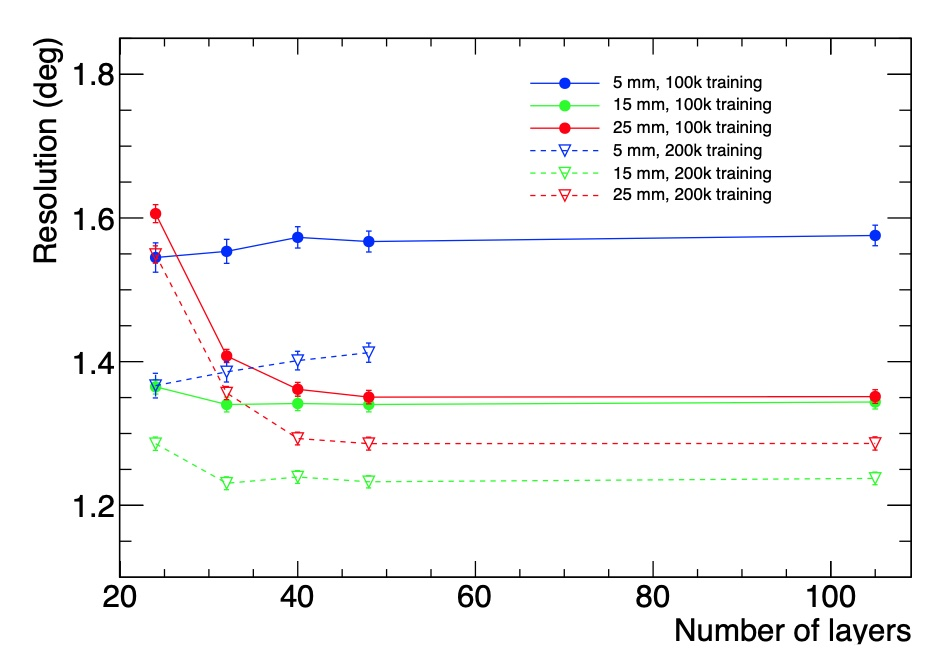
\includegraphics[width=0.48\textwidth]{figures/layer-width.jpg}
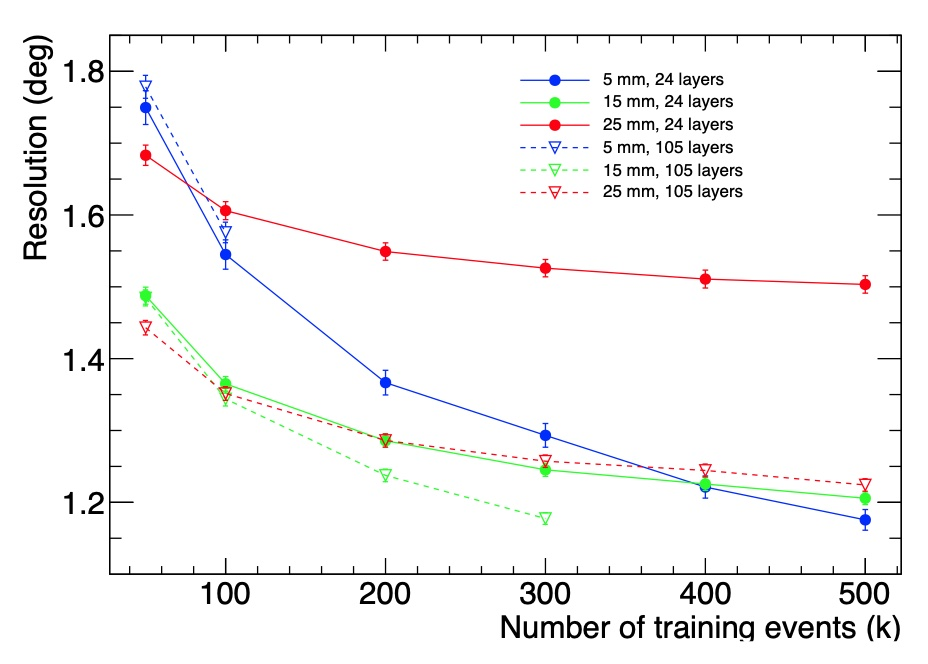
\includegraphics[width=0.48\textwidth]{figures/layer-event.jpg}
\caption{ (Color online) left:Obtained angular resolution for 1 GeV and $\theta_{\rm{true}}=$~10~deg $\gamma$ as a function of number of layers used for reconstruction for 3 different strip widths when the number of trained sample is $2 \times 10^5$. right: Dependence on the number of training samples for using only the first 24 layers (open markers) and full-scaled one(closed markers).
}
\label{fig:multi-parameter}
\end{figure}

%We can place a 5Xo-thick sampling calorimeter for angle measurement in front of a main calorimeter measuring energy of $\gamma$, and obtained angle information with resolution closed to the intrinsic value. 

%angular resolution depends on the radiation length used in the angle measurement and the dependence get disappeared with increasing radiation length. The reconstruction with 4.6$X_{0}$, which corresponds to 24 layers, provides 1.3 degree angular resolution.


%We can reconstruct incident angle by using only the front-layer signals. % and check its performance.
%with the same configuration. 
%As signals in front layers are only used, $\gamma$s starting to interact at the rear layers can not be detected and their angles, therefore, can not be reconstructed. To reject such cases, total energy in the front layer is required to be larger than 1\% of incident $\gamma$ energy. Inefficiency due to the selection is estimated to be 5.8\%. 

%the angular resolution is improved larger than 24 layers which corresponds to the 4.6$X_{0}$. With the energy threshold of 10 MeV to the first 24 layers, 94$\%$ of incident gammas are reconstructed correctly, and the remained 6$\%$ do not generate enough shower particles.

%reconstruction with the first 24 layers, which corresponds to the 4.6$X_{0}$, provides the identical resolution with one with the full geometry. The inefficiency can arise mainly due to no responses in the front region, and can be evaluated by comparing the number of events with and without applying the minimum total energy ($E_{\rm{tot}}$) threshold in the front region. The inefficiency for 4.6$X_{0}$ is estimated to be 5.8\%. Figure~\ref{fig:angle_reco_layer} shows the reconstructed $\theta$ distribution (left) and the angular resolution as a function of front layer depth used for the reconstruction (right). The reconstructed $\theta$ distribution without the $E_{\rm{tot}}$ threshold exhibits a delta peak near $\theta=$~0 as a results of failures of the $\theta$ reconstruction, and this peak clearly disappears by applying the $E_{\rm{tot}}$ threshold. The angular resolution is evaluated after applying the $E_{\rm{tot}}$ threshold, and estimated to be 1.3 deg, which is comparable results with fig.~\ref{fig:angle_reco_width} for 4.6$X_{0}$ depth, so that the radiation length for the $\theta$ reconstruction is determined to be 4.6$X_{0}$.

%The angle reconstruction is tested only with signals in front layers. Usages of front-layer signals are applied to the data sample for training and test procedures at the same time. The reconstruction with 24 layers, which possess 4.6$X_{0}$, provides the identical resolution with one with the full geometry. The inefficiency can arise mainly due to no responses in the front region, and can be evaluated by comparing the number of events with and without applying the minimum total energy ($E_{\rm{tot}}$) threshold in the front region. The inefficiency for 4.6$X_{0}$ is estimated to be 5.8\%. Figure~\ref{fig:angle_reco_layer} shows the reconstructed $\theta$ distribution (left) and the angular resolution as a function of front layer depth used for the reconstruction (right). The reconstructed $\theta$ distribution without the $E_{\rm{tot}}$ threshold exhibits a delta peak near $\theta=$~0 as a results of failures of the $\theta$ reconstruction, and this peak clearly disappears by applying the $E_{\rm{tot}}$ threshold. The angular resolution is evaluated after applying the $E_{\rm{tot}}$ threshold, and estimated to be 1.3 deg, which is comparable results with fig.~\ref{fig:angle_reco_width} for 4.6$X_{0}$ depth, so that the radiation length for the $\theta$ reconstruction is determined to be 4.6$X_{0}$.

%\begin{figure}[!hbt]
%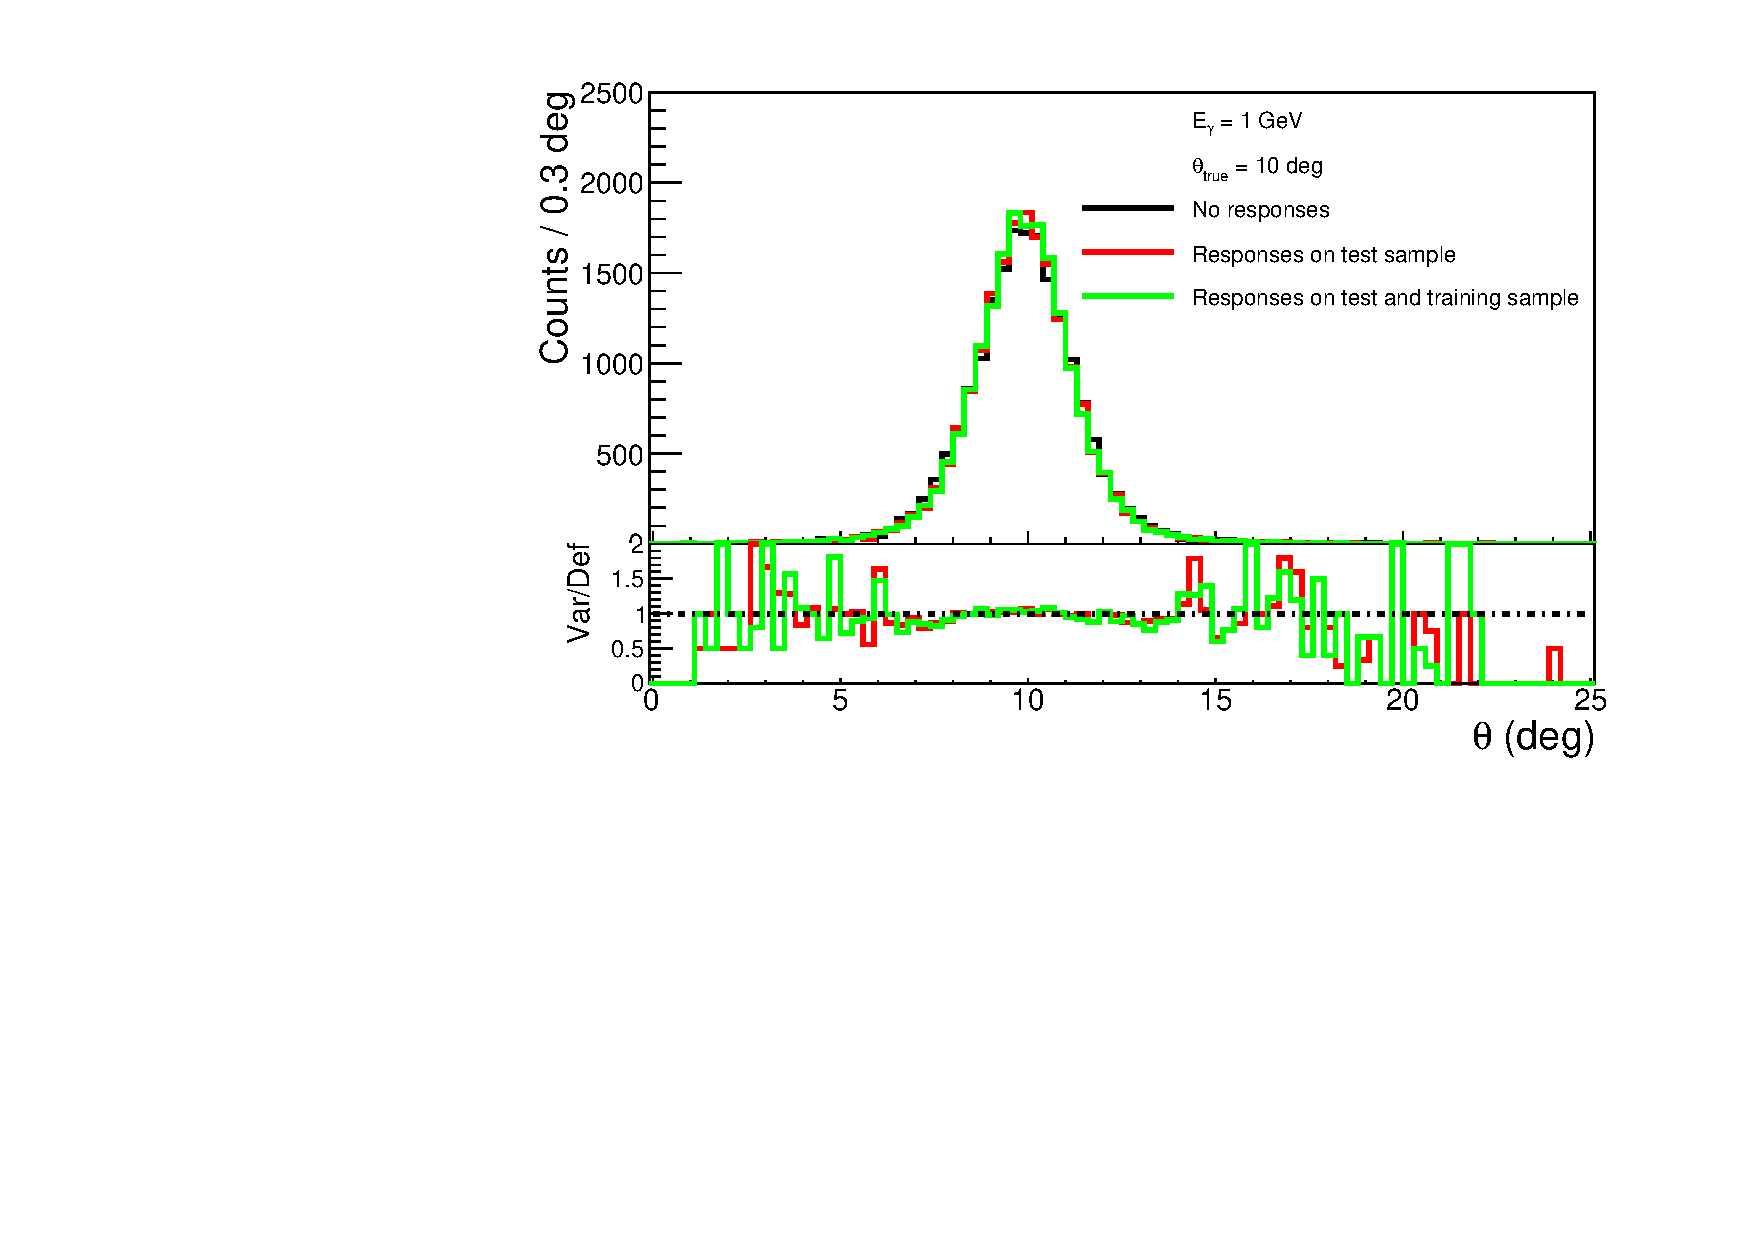
\includegraphics[width=0.8\textwidth]{figures/Fig4_reco_ecut.pdf}
%\caption{ (Color online) Reconstructed $\theta$ before (black) and after (red and green) applying the responses related with the energy measurement. The red (green) distribution is constructed with the training samples without (with) such effects and the test samples with such effects. Simulated effects are found to be not significant.}
%\label{fig:angle_reco_ecut}
%\end{figure}

%- Threshold effect 

%\subsection{Expected performance}

%- W-Fiber 

%- Attenuation effect (NIM A715, pp48-55 (2013))

%- Light Yield (40/1mm $\rightarrow$ 200/MeV (UCV) other reference ?)


%The detector responses on the energy deposit are studied. The attenuation effect, smearing effect due to the photon statistics, and energy threshold for each channel are considered. The attenuation effect is applied to the deposit energy in each channel with the attenuation function, described in~\cite{Murayama:2020mcp}. The coefficients for the attenuation effect are assumed to be same with~\cite{Murayama:2020mcp}. The energy deposit after the attenuation effect is smeared with respect to the number of photon statistics. The number of photons ($\rm{n.p.e}$) is assumed to be 50 for 1 MeV. The standard deviation ($\sigma(E)$) for the smearing can be defined as 

%\begin{eqnarray}
%\sigma(E) = \sqrt{E/\rm{n.p.e}}
%\end{eqnarray}
%After the smearing attenuated energy deposit, the energy threshold (0.5 MeV) is applied to the all channels. These effects are applied to the test samples and the training samples, and the training is done with and without applying such effects and the test is done with applying the effects. Figure~\ref{fig:angle_reco_ecut} shows that the angular resolution is found to be not significant against such effects.

%\begin{figure}[!hbt]
%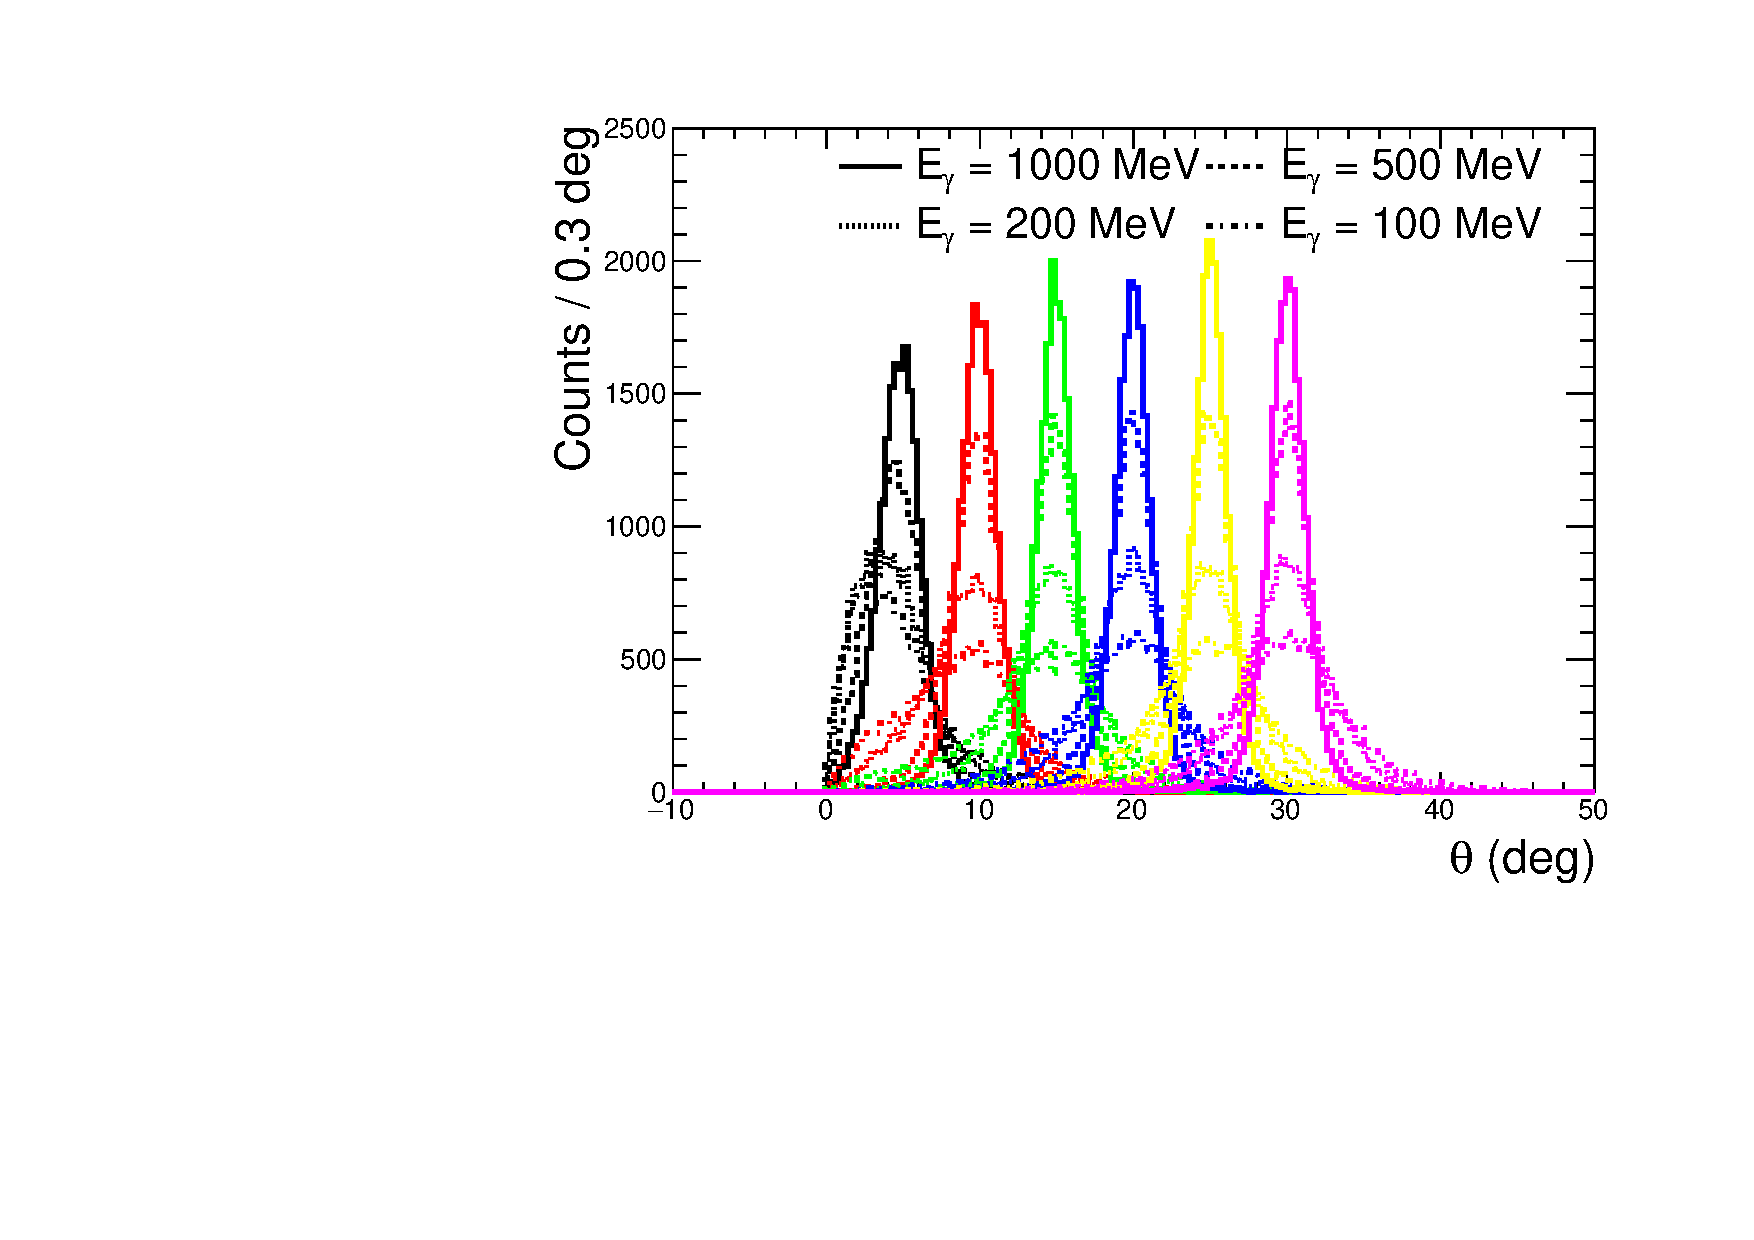
\includegraphics[width=0.6\textwidth]{figures/Fig5_reco_hist.pdf}
%\caption{ (Color online) Reconstructed $\theta$ with respect to each true incident $\theta$ and true %$\gamma$ energy. The incident $\theta_{\rm{true}}$ is illustrated with different colors, which are explained in fig.\ref{fig:angle_reco_def}, and the $\gamma$ energy is illustrated with different lines.}
%\label{fig:angle_reco_dep}
%\end{figure}

%The $\theta$ reconstruction dependencies on the incident angle and the incident energy are studied. Figure~\ref{fig:angle_reco_dep} shows the reconstructed $\theta$ with respect to the incident angle and the incident energy with different line colors and styles. The incident angle dependence of the reconstruction is found to be not significant for higher $E_{\gamma}>$~500~MeV and appears at lower $E_{\gamma}=$~200~MeV. The dependence on the incident energy can be clearly seen for all $\theta_{\rm{true}}$. The reconstruction for $\theta_{\rm{true}}=$~5~deg with lower $E_{\gamma}<$~200~MeV has a shifted maximum point due to their large standard deviations.

\section{SUMMARY}
\label{sec:sum}
We studied a possibility to measure incident angle of the medium-energy $\gamma$ by using a finely segmented sampling calorimeter. With the configuration of alternation 1-mm thick lead sheets and 5-mm thick plastic scintillators, it will measure the energy for 1-GeV $\gamma$ with 4$\%$ of resolution which is mainly determined by the sampling fluctuation. 

For the angular measurement, we need to optimize detector configuration such as width of strips and number of layers. Also, the angular resolution is strongly depends on the goodness of the training of the $\XGB$ which depends on the number of training sample. For a case study of 15-mm strip width and 24 layers, we can achieve the angular resolution as 1.2 degrees with 94$\%$ efficiency. It depends on the incident energy of the $\gamma$, which will limit strictly on the applicable ranger of the measurement. 

On the other hand, there are three major parameters to determine the performance of the measurement. With detailed studies on the optimization of the parameters, it would be possible to design the detector to satisfy the experimental requirement in various studies. 

%Still there are many sources o

%When we focus only on the angle measurement, the first 24 layers (4.6 Xo) provide a resolution as that of the full geometry (20 Xo) with 94$\%$ of detection efficiency. The angular resolution is not changed significantly increasing the width of the strips up to 25mm and expected to be 1.2 degrees for the 1 GeV gamma.

%https://github.com/chenkkkk/MTR-TSF

\label{sec:con}


%\pagebreak

\begin{acknowledgments}
\end{acknowledgments}

\bibliography{paper}

\end{document}
